\documentclass[masc,grad]{coppe} %Universal input encoding G.L.
% \documentclass[aprovado,masc,grad]{coppe} %Universal input encoding G.L.
\maxdeadcycles=20
\usepackage[utf8]{inputenc}
\usepackage[english]{babel}
% \usepackage[brazil]{babel}
\usepackage[T1]{fontenc}
\usepackage{graphicx}
\usepackage{pax}
\usepackage{tikzscale}
\usepackage{appendix}
\usepackage{pgfplots}
\pgfplotsset{compat=newest}
\usepgfplotslibrary{groupplots}
\usepgfplotslibrary{dateplot}
\usepackage{xargs}
\usepackage{rotating}
\usepackage{pdflscape}
\usepackage{afterpage}
\usepackage[paper=A4,pagesize]{typearea}
\graphicspath{{../../figures/}} 
\usepackage{subcaption} 
\usepackage{hyperref}
\usepackage{amsmath,amssymb} 
\usepackage{indentfirst}
\usepackage[algo2e,linesnumbered,ruled]{algorithm2e}
\usepackage{algorithmic}
%%If desirable, the user can enable Times New Roman Fonts by uncommenting the next line. G.L.
% \usepackage{mathptmx}
\usepackage{pdfpages}
\usepackage{multirow}
\usepackage{color}
\usepackage{blindtext}
\usepackage{float}
\usepackage{nameref}
\usepackage{cleveref}
\usepackage{multicol}
\usepackage{listings}
\usepackage{enumerate}
\usepackage[acronym,toc]{glossaries}\makeglossaries
\usepackage{tikz}
\usepackage{ladder} %https://github.com/AurelienC/tex-ladder/blob/master/ladder.sty
\usetikzlibrary{arrows,shapes,automata,petri,external,arrows.meta}
	\tikzset{
	place/.style={
	circle,
	thick,
	draw=black!100, % draw=blue!75,
    % fill=blue!20,
    minimum size=6mm
  },
  extPlace/.style={
    circle,
    dotted,
    draw=black!100, % draw=blue!75,
    % fill=blue!20,
    minimum size=6mm
  },
  extTransition/.style={
    rectangle,
    dotted,
    fill=white,
    minimum width=8mm,
    inner ysep=0.7pt
  },
  transition/.style={
    rectangle,
    thick,
    fill=black,
    minimum width=8mm,
    inner ysep=0.7pt
  },
  extTimedtransition/.style={
    rectangle,
    dotted,
    fill=white,
    minimum width=8mm,
    inner ysep=2pt
  },
  timedtransition/.style={
    rectangle,
    thick,
    fill=white,
    minimum width=8mm,
    inner ysep=2pt
  },
  inhibitor/.style={-o},
  text/.style={}
}

\makeatletter
\tikz@def@grow@tokens{2}{1}{-1.5}{0}
\tikz@def@grow@tokens{2}{2}{1.5}{0}
% \tikz@def@grow@tokens{3}{1}{-1}{0}
% \tikz@def@grow@tokens{3}{2}{0}{1}
% \tikz@def@grow@tokens{3}{3}{1.5}{-1}
\makeatother


\definecolor{darkblue}{rgb}{0,0,0.3}
\definecolor{blue}{rgb}{0,0,0.5}
\definecolor{color1}{rgb}{1,0.2,0.3}
\definecolor{color2}{rgb}{0.05490196078,0.41176470588,0.13333333333}
% rgb(14, 105, 34)

\definecolor{color3}{rgb}{0.2,0.2,0.8}
% hyperref setup
\hypersetup{
  % pdftitle={\title},
  pdfauthor={Rafael Accácio Nogueira},
  pdfcreator={Rafael Accácio Nogueira},     
  bookmarksopen=true,         
  bookmarksopenlevel=1,       
  colorlinks=true, % false => boxes 
  linkcolor=blue,
  filecolor=red,  
  urlcolor=blue,  
  citecolor=blue,              
  pdfstartview=Fit,          
  pdfpagemode=UseOutlines,    % this is the option you were lookin for
  pdfpagelayout=TwoPageRight,
}

\makeatletter
\let\stdchapter\chapter
\renewcommand*\chapter{%
  \@ifstar{\starchapter}{\@dblarg\nostarchapter}}
\newcommand*\starchapter[1]{\stdchapter*{#1}}
\def\nostarchapter[#1]#2{
  \stdchapter[#1]{\protect\hyperlink{tocsection}{#1}}}
\makeatother

\makeatletter
\let\stdsection\section
\renewcommand*\section{%
  \@ifstar{\starsection}{\@dblarg\nostarsection}}
\newcommand*\starsection[1]{\stdsection*{#1}}
\def\nostarsection[#1]#2{
  \stdsection[#1]{\protect\hyperlink{tocsection}{#1}}}
\makeatother

\makeatletter
\let\stdsubsection\subsection
\renewcommand*\subsection{%
  \@ifstar{\starsubsection}{\@dblarg\nostarsubsection}}
\newcommand*\starsubsection[1]{\stdsubsection*{#1}}
\def\nostarsubsection[#1]#2{
  \stdsubsection[#1]{\protect\hyperlink{tocsection}{#1}}}
\makeatother

\makeatletter
\let\stdsubsubsection\subsubsection
\renewcommand*\subsubsection{%
  \@ifstar{\starsubsubsection}{\@dblarg\nostarsubsubsection}}
\newcommand*\starsubsubsection[1]{\stdsubsubsection*{#1}}
\def\nostarsubsubsection[#1]#2{
  \stdsubsubsection[#1]{\protect\hyperlink{tocsection}{#1}}}
\makeatother

\let\oldtoc\tableofcontents
\renewcommand{\tableofcontents}{\pagebreak\hypertarget{tocsection}{}\label{tocsection}\oldtoc}


\newcommand{\figplaceholder}[2]{
	\begin{figure}[H]
		\begin{center}	
			\rule{8cm}{8cm}
			\caption{\todo[FORGOT TO INCLUDE FIGURE]{#1 (placeholder)}}
			\label{fig:#2}
		\end{center}
	\end{figure}
}

\newif\ifdebug
\newcommand{\draft}{\debugtrue}
\newcommand{\final}{\debugfalse}
\newcommand{\todo}[2][FORGOT TO DO SOMETHING]{\ifdebug {\color{red}#2}\else \PackageError{}{#1}{}\fi}
\newcommand\doing[1]{\ifdebug {\color{blue}#1}\else \PackageError{}{FORGOT TO DO SOMETHING}{}\fi}
\newcommand\warning[1]{\ifdebug {\color{red}#1}\fi}
\newcommand\note[1]{\ifdebug {\color{orange}#1}\fi}

\usepackage{fancyhdr}
\pagestyle{fancy}

\fancyhead[L]{\warning{DRAFT}}
\fancyhead[R]{\warning{DEBUG ON}}

\fancyfoot[L]{\warning{TURN DEBUG OFF}}
\fancyfoot[R]{\warning{DRAFT}}

\newtheorem{theorem}{Theorem}
\numberwithin{theorem}{chapter}

\newtheorem{example}{Example}
\numberwithin{example}{chapter}

\newtheorem{definition}{Definition}
\numberwithin{definition}{chapter}

\newtheorem{observation}{Remark}
\numberwithin{observation}{chapter}

\usepackage[export]{adjustbox}

\newcommand{\includetikzfigure}[2][]{
    \ifdebug {\includegraphics[#1]{#2.pdf}}
    \else  \includegraphics[#1]{#2}\fi
}

\newcommand{\addtikzfigureLandscape}[4][width=0.8\textwidth]{
\KOMAoptions{paper=landscape}
\recalctypearea
  \vspace*{\fill}
  \begin{figure}[H]
    \centering
    \ifdebug {\includegraphics[#1]{#2.pdf}}
    \else  \includegraphics[#1]{#2}\fi
    \caption{#3}
    \label{fig:#4}
  \end{figure}
  \vspace*{\fill}
\KOMAoptions{paper=portrait}
\recalctypearea
}

\newcommand{\addtikzfigureLandscapeAthree}[4][width=0.8\textwidth]{
\KOMAoptions{paper=a3,paper=landscape}
% \KOMAoptions{paper=landscape}
\recalctypearea
  \begin{figure}[H]
    \vspace{-2cm}
    \centering
    \ifdebug {\centerline{\includegraphics[#1]{#2.pdf}}}
    \else  \centerline{\includegraphics[#1]{#2}}
\fi
    % \caption{#3}
    % \label{fig:#4}
  \end{figure}
\KOMAoptions{paper=a4,paper=portrait}
\recalctypearea
}

% \newcommand{\addtikzfigureVertCent}[3]{
% \KOMAoptions{paper=landscape}
% \recalctypearea
% % \begin{landscape}
% \vspace*{\fill}
%   \begin{figure}[H]
%     % \centering
%     % \resizebox{\hsize}{!}{
%     % \input{#1}
%      \includegraphics[width=1.15\textwidth]{#1}
%     % }
%     \caption{#2}
%     \label{fig:#3}
%   \end{figure}
% \vspace*{\fill}
% % \end{landscape}
% \KOMAoptions{paper=portrait}
% \recalctypearea
% }

\newcolumntype{P}[1]{>{\centering\arraybackslash}p{#1}}
\newcolumntype{M}[1]{>{\centering\arraybackslash}m{#1}}
\definecolor{keywordstyle}{rgb}{0,0,0.82}
\definecolor{commentstyle}{rgb}{0,0.6,0}
\definecolor{numberstyle}{rgb}{0.5,0.5,0.5}
\definecolor{stringstyle}{rgb}{0.58,0,0.82}

% Listing options
\lstset{ 
  % backgroundcolor=\color{white},   % choose the background color; you must add \usepackage{color} or \usepackage{xcolor}; should come as last argument
  basicstyle=\footnotesize,        % the size of the fonts that are used for the code
  breakatwhitespace=false,         % sets if automatic breaks should only happen at whitespace
  breaklines=true,                 % sets automatic line breaking
  captionpos=t,                    % sets the caption-position to bottom
  commentstyle=\color{commentstyle},    % comment style
  deletekeywords={...},            % if you want to delete keywords from the given language
  escapeinside={\%*}{*)},          % if you want to add LaTeX within your code
  extendedchars=true,              % lets you use non-ASCII characters; for 8-bits encodings only, does not work with UTF-8
  % firstnumber=1000,                % start line enumeration with line 1000
  % frame=single,	                   % adds a frame around the code
  keepspaces=true,                 % keeps spaces in text, useful for keeping indentation of code (possibly needs columns=flexible)
  keywordstyle=\color{keywordstyle},       % keyword style
  % language=Octave,                 % the language of the code
  morekeywords={*,...},            % if you want to add more keywords to the set
  numbers=left,                    % where to put the line-numbers; possible values are (none, left, right)
  numbersep=10pt,                   % how far the line-numbers are from the code
  numberstyle=\tiny\color{numberstyle}, % the style that is used for the line-numbers
  rulecolor=\color{black},         % if not set, the frame-color may be changed on line-breaks within not-black text (e.g. comments (green here))
  showspaces=false,                % show spaces everywhere adding particular underscores; it overrides 'showstringspaces'
  showstringspaces=false,          % underline spaces within strings only
  showtabs=false,                  % show tabs within strings adding particular underscores
  stepnumber=2,                    % the step between two line-numbers. If it's 1, each line will be numbered
  stringstyle=\color{stringstyle},     % string literal style
  tabsize=2,	                   % sets default tabsize to 2 spaces
  title=\lstname                   % show the filename of files included with \lstinputlisting; also try caption instead of title
}

%% as seen in https://tex.stackexchange.com/a/183682/143332
\makeatletter
\newcommand\Autoref[1]{\@first@ref#1,@}
\def\@throw@dot#1.#2@{#1}% discard everything after the dot
\def\@set@refname#1{%    % set \@refname to autoefname+s using \getrefbykeydefault
    \edef\@tmp{\getrefbykeydefault{#1}{anchor}{}}%
    \xdef\@tmp{\expandafter\@throw@dot\@tmp.@}%
    \ltx@IfUndefined{\@tmp autorefnameplural}%
         {\def\@refname{\@nameuse{\@tmp autorefname}s}}%
         {\def\@refname{\@nameuse{\@tmp autorefnameplural}}}%
}
\def\@first@ref#1,#2{%
  \ifx#2@\autoref{#1}\let\@nextref\@gobble% only one ref, revert to normal \autoref
  \else%
    \@set@refname{#1}%  set \@refname to autoref name
    \@refname~\ref{#1}% add autoefname and first reference
    \let\@nextref\@next@ref% push processing to \@next@ref
  \fi%
  \@nextref#2%
}
\def\@next@ref#1,#2{%
   \ifx#2@ and~\ref{#1}\let\@nextref\@gobble% at end: print and+\ref and stop
   \else, \ref{#1}% print  ,+\ref and continue
   \fi%
   \@nextref#2%
 }
 \makeatother

\newcommand{\colvec}[2][1]{%
  \scalebox{#1}{%
    \renewcommand{\arraystretch}{.7}%
    $\begin{bmatrix}#2\end{bmatrix}$%
  }
}


%%% Local Variables:
%%% mode: latex
%%% TeX-master: "./monografia.tex"
%%% End:

% \usepackage{fontspec}
% \usepackage{fontawesome}
\newcommandx\acr[5][4=,5=]{
  \ifthenelse{\equal{#5}{}}
  {
    \acrSing{#1}{#2}{#3}
  }
  {
    \acrPl{#1}{#2}{#3}{#4}{#5}
  }
  } 

\newcommand{\acrSing}[3]{\newacronym{#1}{#2}{#3}
  \expandafter\newcommand\csname #1\endcsname{\gls{#1}}}

\newcommand{\acrPl}[5]{
  \newacronym[plural=#4,firstplural=#5 (#4)]{#1}{#2}{#3}
  \expandafter\newcommand\csname #1\endcsname{\gls{#1}}
  \expandafter\newcommand\csname #4\endcsname{\glspl{#1}}
}

\renewcommand{\symbl}[3]{\newglossaryentry{#1}{name ={#2},	description ={#3}}
  \expandafter\newcommand\csname #1\endcsname{\gls{#1}}
}


\newglossarystyle{dottedlocations}{%
   \glossarystyle{list}%
   \renewcommand*{\glossaryentryfield}[5]{%
   \item[\glsentryitem{##1}\glstarget{##1}{##2}] ##3, p %
       \unskip\leaders\hbox to 2.9mm{} ##5}%
   \renewcommand*{\glsgroupskip}{}%
}

 \newglossarystyle{acronyms}{%
 % put the glossary in the itemize environment:
 \renewenvironment{theglossary}%
   {\begin{tabbing}}{\end{tabbing}}%
 % have nothing after \begin{theglossary}:
 \renewcommand*{\glossaryheader}{}%
 % have nothing between glossary groups:
 \renewcommand*{\glsgroupheading}[1]{}%
 \renewcommand*{\glsgroupskip}{}%
 % set how each entry should appear:
 \renewcommand*{\glossentry}[2]{%
 \glstarget{##1}{\glossentryname{##1}}\\% \kill % the entry name
 \=\glossentrysymbol{##1}% the symbol in brackets
 \space \glossentrydesc{##1},% the description
 \space p. ##2\\% the number list in square brackets
 }%
 % set how sub-entries appear:
 \renewcommand*{\subglossentry}[3]{%
   \glossentry{##2}{##3}}%
}


 \newglossarystyle{symbols}{%
 % put the glossary in the itemize environment:
 \renewenvironment{theglossary}%
   {\begin{tabbing}}{\end{tabbing}}%
 % have nothing after \begin{theglossary}:
 \renewcommand*{\glossaryheader}{}%
 % have nothing between glossary groups:
 \renewcommand*{\glsgroupheading}[1]{}%
 \renewcommand*{\glsgroupskip}{}%
 % set how each entry should appear:
 \renewcommand*{\glossentry}[2]{%
 \glstarget{##1}{\glossentryname{##1}}\\% \kill % the entry name
 \=\textbf{\glossentrysymbol{##1}}% the symbol in brackets
 
 \space \glossentrydesc{##1},% the description
 \space p. ##2\\% the number list in square brackets
 }%
 % set how sub-entries appear:
 \renewcommand*{\subglossentry}[3]{%
   \glossentry{##2}{##3}}%
 }


\acr{DAOCT}{DAOCT}{Deterministic Automaton
  with Outputs and Conditional Transitions}
\acr{ECA}{ECA}{Engenharia de controle e Automação}
\acr{PLC}{PLC}{Programmable Logic Controller}
[PLCs][Programmable Logic Controllers]
\acr{DES}{DES}{Discrete Event System}
[DESs][Discrete Event Systems]


\acr{LD}{LD}{Ladder Diagram}

\acr{CIPN}{CIPN}{Control Interpreted Petri Net}

% DAOCT
\symbl{OmegaSet}{$\Omega$}{$\Omega \subset \mathbb{N}_1^{m_i + m_0}$ Set of IO vectors}
\symbl{SigmaSet}{$\Sigma$}{Set of events}
\symbl{XSet}{$X$}{Set of states}
\symbl{ffunction}{$f$}{$f : X \times \Sigma^* \rightarrow X$ Deterministic
  transition function}
\symbl{lambdafunction}{$\lambda$}{$\lambda : X \rightarrow \Omega$ State
  output function}
\symbl{RSet}{$R$}{$R = \{1,2,\dots,r\} $ Set of path indices}
\symbl{thetafunction}{$\theta$}{$\theta : X \times \Sigma \rightarrow 2^R$ Path
  estimation function}
\symbl{xZero}{$x_0$}{Initial State}
\symbl{XfSet}{$X_f$}{$X_f \subseteq X$ Set of final states}
%%% Local Variables:
%%% mode: latex
%%% TeX-master: "./monografia.tex"
%%% End:
\makeindex
\makelosymbols
\makeloabbreviations

% \final
\draft

% include only to speed up tests
% \includeonly{test/examples}
\signedFrontPage{../../figures/poli-logo.pdf}

	



\usetikzlibrary{arrows,shapes,petri,external,arrows.meta}
	\tikzset{
	place/.style={
	circle,
	thick,
	draw=black!100, % draw=blue!75,
    % fill=blue!20,
    minimum size=6mm
  },
  extPlace/.style={
    circle,
    dotted,
    draw=black!100, % draw=blue!75,
    % fill=blue!20,
    minimum size=6mm
  },
  extTransition/.style={
    rectangle,
    dotted,
    fill=white,
    minimum width=8mm,
    inner ysep=0.7pt
  },
  transition/.style={
    rectangle,
    thick,
    fill=black,
    minimum width=8mm,
    inner ysep=0.7pt
  },
  extTimedtransition/.style={
    rectangle,
    dotted,
    fill=white,
    minimum width=8mm,
    inner ysep=2pt
  },
  timedtransition/.style={
    rectangle,
    thick,
    fill=black,
    minimum width=8mm,
    inner ysep=2pt
  },
  inhibitor/.style={-o},
  text/.style={}
}

\begin{document}





% Identificação e Detecção de Falhas em um Sistema de Manufatura Didático
\title{Identification and Failure~Detection in a Didactic~Manufacture~System}
\foreigntitle{Identificação e Detecção~de~Falhas em um Sistema~de~Manufatura~Didático}
\author{Rafael Accácio}{Nogueira}

\advisor{Prof.}{Marcos Vicente de Brito}{Moreira}{D.Sc.}

% Case advisor is a woman add {f} Example:
% \advisor{Prof.}{Marie}{Sklodowksca-Curie}{PhD.}{f}

% \advisor{Prof.}{Nome do Segundo Orientador}{Sobrenome}{Ph.D.}
% \advisor{Prof.}{Nome do Terceiro Orientador}{Sobrenome}{D.Sc.}

\examiner{Prof.}{Marcos Vicente de Brito Moreira}{D.Sc.}
% \examiner{Prof.}{Fernando César Lizarralde}{D.Sc.}
% \examiner{Prof.}{Nome do Terceiro Examinador Sobrenome}{D.Sc.}
\department{ECA}

\date{04}{2019}
% \newfontfamily{\FA}{FontAwesome}

\keyword{Failure~Detection}
\keyword{Discrete~Event~Systems}

\maketitle
\frontmatter
\makefrontpage
\makecatalog

% \def\Github{{\FA \faGithub}}
% \href{http://github.com/Accacio}{\Github Accacio}
\dedication{“It's a dangerous business going out your door. You step onto the road,
and if you don't keep your feet, there's no knowing where you might be swept off
to.” \\(J.R.R Tolkien)}
% ``É um negócio perigoso, Frodo, sair da sua porta. Você pisa na estrada, e, se
% não controlar seus pés, não há como saber até onde você pode ser levado''
% ``Se enxerguei mais longe, foi porque me apoiei sobre os ombros de gigantes.'' (Isaac Newton)

%%% Local Variables:
%%% mode: latex
%%% TeX-master: "../monografia.tex"
%%% End:


\chapter*{Agradecimentos}
\chapter*{Agradecimentos} Primeiramente a Deus, sem
quem nada é possível e por \mbox{\textbf{todas}} as pessoas colocadas em meu caminho, que
me fizeram crescer e ser o indivíduo que hoje sou.

Aos meus pais, Rosemeri e Rogério. Por todo amor, carinho, atenção e
apoio dados, pela primeira educação, essencial para toda minha
trajetória, educação não só acadêmica, mas também moral. Obrigado, por tudo ! Amo muito vocês.

A todas minhas professoras e professores por 
 mostrarem o quão importante e bonita é a profissão e por terem sempre
 instigado a sede pelo aprendizado. Agradeço àqueles que contribuíram para
 minha base acadêmica e profissional.

As amizades que fiz, as que se foram de minha convivência e
   as que permaneceram, agradeço aqueles que conheci na UFRJ, mais especificamente a nossa turma T17,
   pois se chegamos até onde chegamos foi porque estivemos juntos, fortes, ombro
   no ombro, tentando não deixar o outro cair, mas quando alguém caía
   sempre uma mão amiga se estendia para ajudar a levantar e recomeçar. 

Ao Paulo Yamasaki, pelo convívio no LABECA, e pelas
   trocas de ideias em assuntos gerais que por fim, intencionalmente ou não, se
   tornariam orientação em diversos projetos que fiz na faculdade, e até mesmo
   orientação acadêmica e profissional. 

Aos melhores companheiros de grupo, Gabriel Pelielo e Rodrigo Moysés, um
verdadeiro ``Power Trio''. Também a Philipe Moura e Felipe Matheus, que me
incentivaram a sair da minha zona de conforto e me fizeram compreender de fato o sentido do quão
``perigoso'' é sair pela porta de casa, pois quando saímos da nossa zona de
conforto, coisas mágicas podem acontecer e pessoas mágicas podem aparecer em
nossas vidas.

À Evelise, a pessoa mágica que apareceu em minha vida, que me ajudou
fisicamente e psicologicamente nos momentos que mais precisei. Obrigado por escolher compartilhar parte de sua
vida comigo e por toda a força dada para o término desse ciclo. Eu te amo!  

Por fim às pessoas que me ajudaram mais diretamente neste projeto, Ryan
Pitanga e ao meu orientador Marcos Moreira 

%%% Local Variables: mode: latex TeX-master: "../monografia.tex" End:


\begin{foreignabstract}

In this work, we present ...

\end{foreignabstract}
\begin{abstract}

Apresenta-se, nesta tese, ...

\end{abstract}

\tableofcontents

\listoffigures
\listoftables
% \printlosymbols
% \printloabbreviations

\printglossary[style=acronyms,title=List of Acronyms,type=\acronymtype]\newpage
\printglossary[style=symbols,title=List of Symbols]

\mainmatter


\chapter{Examples}
\label{chap:examples}

\section{teste}
\subsection{teste}
\subsubsection{teste}
\begin{figure}[H]
  \centering
  \begin{tikzpicture}
    \node[anchor=south west,inner sep=0] (image) at (0,0) {
      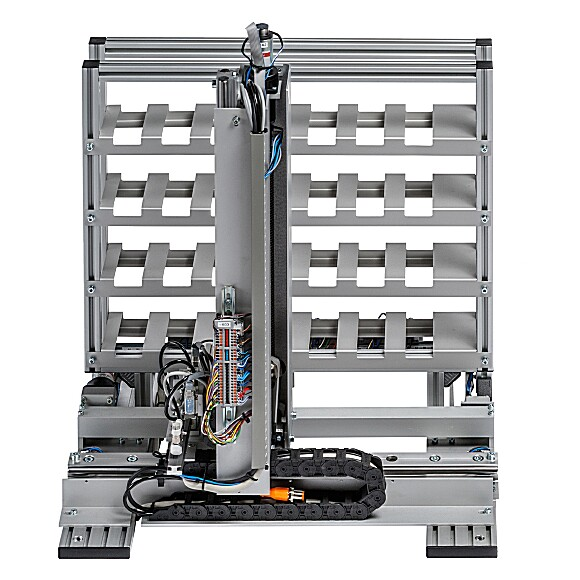
\includegraphics[width=8cm]{maquete/elevador/69523_3.jpg}
    };
    % \draw[red,ultra thick,rounded corners] (0,0) rectangle (9.4,6.2);
    \begin{scope}[x={(image.south east)},y={(image.north west)}]
        % \draw[help lines,xstep=.1,ystep=.1] (0,0) grid (1,1);
        % \foreach \x in {0,1,...,9} { \node [anchor=north] at (\x/10,0) {0.\x}; }
        % \foreach \y in {0,1,...,9} { \node [anchor=east] at (0,\y/10) {0.\y}; }
      \draw[red] (1,0.5) node {\textbf{Right}};
      \draw[red] (0,0.5) node {\textbf{Left}};
      \draw[red] (0.5,1) node {\textbf{Top}};
      \draw[red] (0.5,0) node {\textbf{Bottom}};
      \end{scope}
  \end{tikzpicture}
  \caption{Storage Unit}
\end{figure}


\begin{figure}[H]
  \centering
  \begin{tikzpicture}
    \node[anchor=south west,inner sep=0] (image) at (0,0) {
      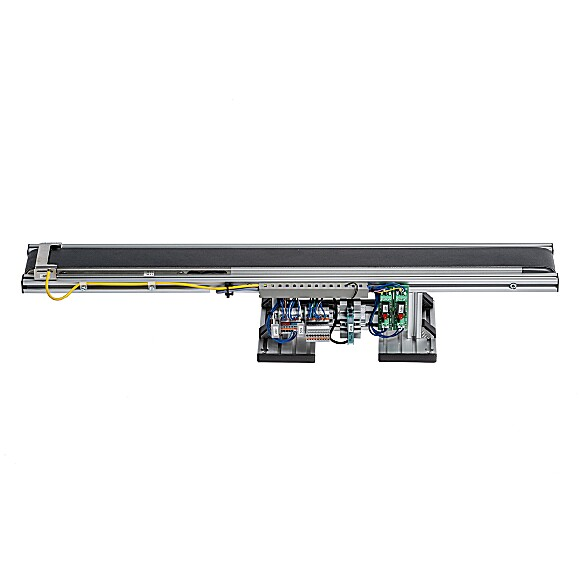
\includegraphics[trim={0 6cm 0 5cm},clip,width=8cm]{maquete/esteira/40778_3.jpg}
    };
    % \draw[red,ultra thick,rounded corners] (0,0) rectangle (9.4,6.2);
    \begin{scope}[x={(image.south east)},y={(image.north west)}]
        % \draw[help lines,xstep=.1,ystep=.1] (0,0) grid (1,1);
        % \foreach \x in {0,1,...,9} { \node [anchor=north] at (\x/10,0) {0.\x}; }
        % \foreach \y in {0,1,...,9} { \node [anchor=east] at (0,\y/10) {0.\y}; }
        \draw [->,>=stealth,red, very thick](0.9,0.7) -- (0.1,0.7);
        \draw [red] (0.5,0.8) node {Forward};
        \draw [->,>=stealth,red, very thick](0.1,0.1) -- (0.9,0.1);
        \draw [red](0.5,0.0) node {Reverse};
      \end{scope}
  \end{tikzpicture}
  \caption{Conveyor Belt}
\end{figure}

\begin{figure}[H]
  \centering
  \begin{tikzpicture}
    \node[anchor=south west,inner sep=0] (image) at (0,0) {
      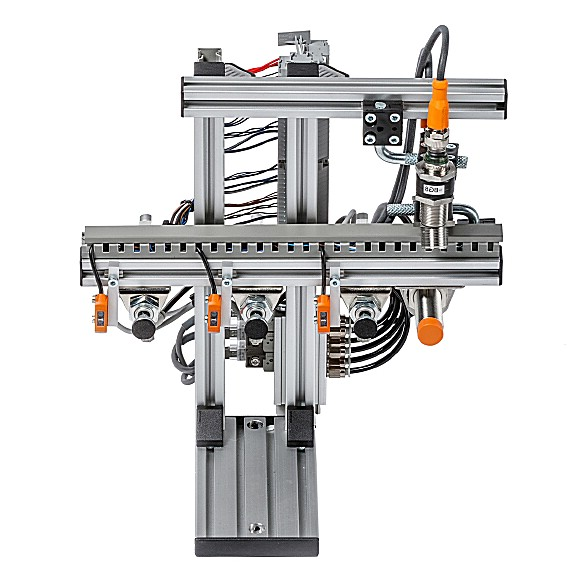
\includegraphics[trim={0 0 0 0},clip,width=8cm]{maquete/sensores/69511_3.jpg}
    };
    % \draw[red,ultra thick,rounded corners] (0,0) rectangle (9.4,6.2);
    \begin{scope}[x={(image.south east)},y={(image.north west)}]
        % \draw[help lines,xstep=.1,ystep=.1] (0,0) grid (1,1);
        % \foreach \x in {0,1,...,9} { \node [anchor=north] at (\x/10,0) {0.\x}; }
        % \foreach \y in {0,1,...,9} { \node [anchor=east] at (0,\y/10) {0.\y};  }
        \draw[red,ultra thick,rounded corners] (0.15,0.4) rectangle ++ (0.15,0.1);
        \draw[red] (0.1,0.1) node {\textbf{Left}};
        \draw[->,>=stealth,red, very thick] (0.2,0.38) -- (0.1,0.15);
        \draw[magenta,ultra thick,rounded corners] (0.35,0.4) rectangle ++ (0.15,0.1);
        \draw[magenta] (0.1,0.8) node {\textbf{Center}};
        \draw[->,>=stealth,magenta, very thick] (0.4,0.52) -- (0.2,0.75);
        \draw[cyan,ultra thick,rounded corners] (0.53,0.4) rectangle ++ (0.15,0.1);
        \draw[cyan] (0.7,0.1) node {\textbf{Right}};
        \draw[->,>=stealth,cyan, very thick] (0.65,0.38) -- (0.7,0.15);
      \end{scope}
  \end{tikzpicture}
  \caption{Sensors}
\end{figure}

\begin{figure}[H]
  \centering
  \begin{tikzpicture}
    \node[anchor=south west,inner sep=0] (image) at (0,0) {
      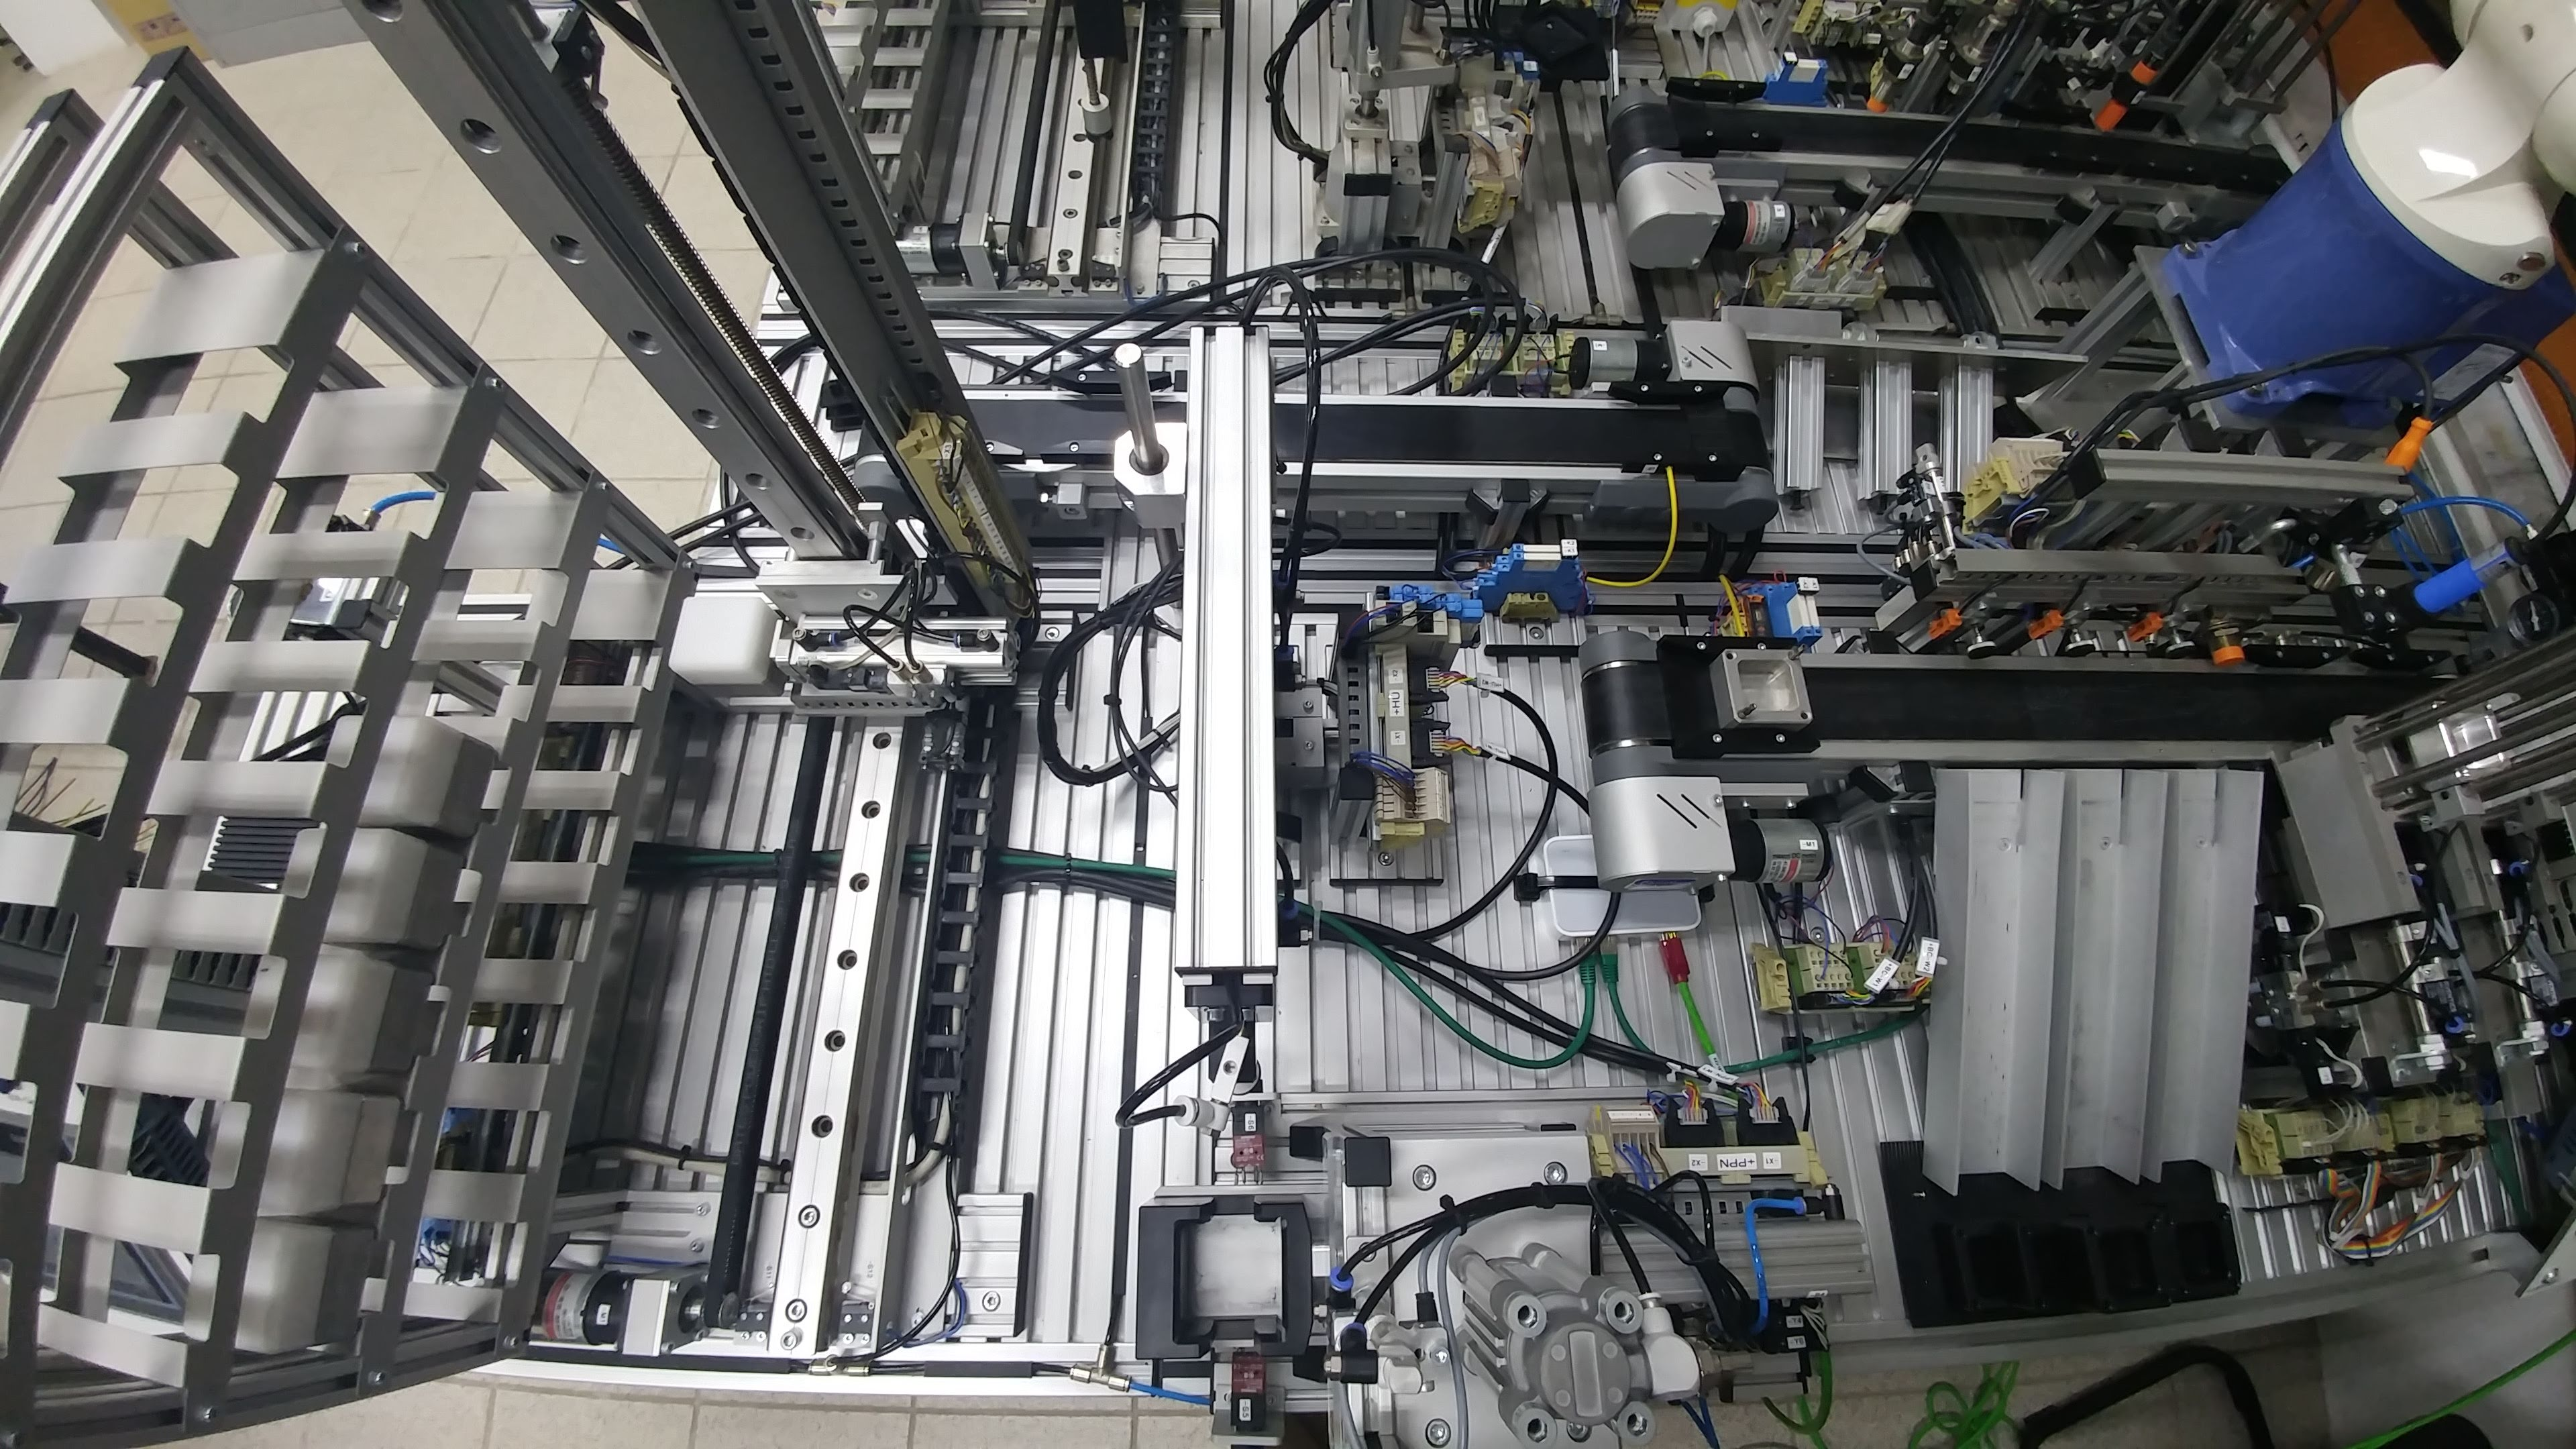
\includegraphics[trim={20cm 0 30cm 20cm},clip,width=0.8\textwidth]{maquete/armAngles.jpg}
    };
    % \draw[red,ultra thick,rounded corners] (0,0) rectangle (9.4,6.2);
    \begin{scope}[x={(image.south east)},y={(image.north west)}]
        % \draw[help lines,xstep=.1,ystep=.1] (0,0) grid (1,1);
        % \foreach \x in {0,1,...,9} { \node [anchor=north] at (\x/10,0) {0.\x}; }
        % \foreach \y in {0,1,...,9} { \node [anchor=east] at (0,\y/10) {0.\y}; }a
        
      
        \draw[red,->,>=stealth,very thick] (0.48,0.9) -- ++(-50:0.7);
        \draw[red,->,>=stealth,very thick] (0.48,0.9) -- ++(-95:0.7);
        \draw[red,->,>=stealth,very thick] (0.48,0.9) -- ++(-120:0.7);

        \draw[fill=red, fill opacity=0.2,draw=none] (0.48,0.9) -- ([shift=(-50:0.5)]0.48,0.9) arc (-50:-95:0.5);
        \draw[fill=blue, fill opacity=0.2,draw=none] (0.48,0.9) -- ([shift=(-95:0.5)]0.48,0.9) arc (-95:-120:0.5);

        \draw [fill,white,fill opacity=0.7,draw=none] (0.02,0.23) rectangle ++ (0.35,0.06);
        \draw [black] (0.2,0.25) node {\tiny \textbf{STORAGE\_ANGLE\_BEFORE}};

        \draw [fill,white,fill opacity=0.7,draw=none] (0.25,0.13) rectangle ++ (0.3,0.06);
        \draw [black] (0.4,0.15) node {\tiny \textbf{PRESS\_ANGLE\_AFTER}};

        \draw [fill,white,fill opacity=0.7,draw=none] (0.7,0.28) rectangle ++ (0.3,0.06);
        \draw [black] (0.85,0.3) node {\tiny \textbf{PRESS\_ANGLE\_BEFORE}};

        \draw [fill,white,fill opacity=0.7,draw=none] (0.1,0.82) rectangle  (0.2,0.96);
        \draw [red,thick] ([shift=(0:0.03)]0.15,0.9) arc (0:180:0.03);
        \draw[black,->,>=stealth,very thick] (0.15,0.85) -- ++(0,0.1);
        \draw [red,->,>=stealth,thick] ([shift=(0:-0.03)]0.15,0.9) arc (-180:-20:0.03);

      \end{scope}
  \end{tikzpicture}
  \caption{Sensors}
\end{figure}

Identification algorithm as seen in \cite{moreira2018enhanced}
\begin{algorithm2e}
  \caption{Identification Algorithm}\label{alg:identification}
\KwIn
{%
Modified observed paths $p_i^k$, for i= 1,\dots,$r$
}
\KwOut
{%
DAOCT = $($\XSet,\SigmaSet,\OmegaSet,\ffunction,\lambdafunction,\RSet,\thetafunction,\xZero,\XfSet$)$
}
\BlankLine
Create an initial state $x_0$, and define $\lambda(x_0) = \tilde{\lambda}(x_0) =
y_{1,1}$

$X = \{ x_0\}, X_f = \emptyset$

\For{$i = 1$ \KwTo $r$}
{
\For{$j = 1$ \KwTo $l_i - 1$}
{
  Find the State $x \in X $ such that $\tilde{\lambda}(x) = y_{i,j+1}$

  \eIf{$\tilde{\lambda}(x) \neq y_{i,j+1}$ for all $ x \in X$}
  { Create state $x^\prime$ and define $\tilde{\lambda}(x^\prime) = y_{i,j+1}$

$X = X \cup \{ x^\prime\}$

$\lambda(x^\prime) = \tilde{\lambda_l}(x^\prime)$

}
{
  Find $x^\prime \in X$ such that $\tilde{\lambda}(x^\prime) = y_{i,j+1}$
}
$f(x,\sigma_{i,j}) = x^\prime$

Add $i$ to $\theta(x,\sigma_{i,j})$

\If{$j = l_i - 1$}
{
  $X_f = X_f \cup \{x^\prime\}$
}
}
}
\end{algorithm2e}

% \begin{table}[H]
%   \centering
%   \caption{table}
%   \begin{tabular}{cc}
%     \label{tab:tab1}
%     \hypertarget{tab:1}{}
%     Transição&Significado\\
%     \hline \\
%     \hyperlink{partialNet:t1}{\hypertarget{partialTable:t1}{$t_{1}$}}&Test\\
%     \hyperlink{partialNet:p1}{\hypertarget{partialTable:p1}{$p_{1}$}}&balbalbal\\
%     \hyperlink{partialNet:p0m2}{\hypertarget{partialTable:p0m2}{$p_{0}$}}&balbalbal
%   \end{tabular}
% \end{table}

% \newpage
% \begin{figure}[h]
%   \centering
%   \begin{tikzpicture}[>=latex',line join=bevel,]
%%
\node (p0m2) at (27.0bp,18.0bp) [draw,ellipse,place, tokens=2, label=above:, label=left:\hyperlink{partialTable:p0m2}{\hypertarget{partialNet:p0m2}{$p_{0}$}},rotate=90] {};
  \node (tt1) at (114.0bp,18.0bp) [draw,ellipse,timedtransition, label=above:, label=left:\hyperlink{partialTable:tt1}{\hypertarget{partialNet:tt1}{$t_{1}$}},rotate=90] {};
  \node (ep1) at (185.0bp,18.0bp) [draw,ellipse,extPlace, label=above:, label=left:\hyperlink{partialNet:p1}{$p_{1}$},rotate=90] {};
  \draw [-Latex,inhibitor] (p0m2) ..controls (54.05bp,18.0bp) and (76.966bp,18.0bp)  .. (tt1);
  \definecolor{strokecol}{rgb}{0.0,0.0,0.0};
  \pgfsetstrokecolor{strokecol}
  \draw (70.5bp,27.0bp) node {3};
  \draw [-Latex] (tt1) ..controls (141.25bp,18.0bp) and (147.94bp,18.0bp)  .. (ep1);
%
\end{tikzpicture}

%   \caption{example }
%   \label{fig:example}
% \end{figure}

% \newpage
% \begin{figure}[h]
%   \centering
%   \begin{tikzpicture}[>=latex',line join=bevel,]
%%
\node (et1) at (27.0bp,18.0bp) [draw,ellipse,extTransition, label=above:, label=left:\hyperlink{partialNet:t1}{$t_{1}$},rotate=90] {};
  \node (p1) at (95.0bp,18.0bp) [draw,ellipse,place, label=above:, label=left:\hyperlink{partialTable:p1}{\hypertarget{partialNet:p1}{$p_{1}$}},rotate=90] {};
  \draw [-Latex] (et1) ..controls (54.266bp,18.0bp) and (57.727bp,18.0bp)  .. (p1);
%
\end{tikzpicture}

%   \caption{example }
%   \label{fig:example}
% \end{figure}

% \newpage

% \begin{figure}[H]
%   \centering
%   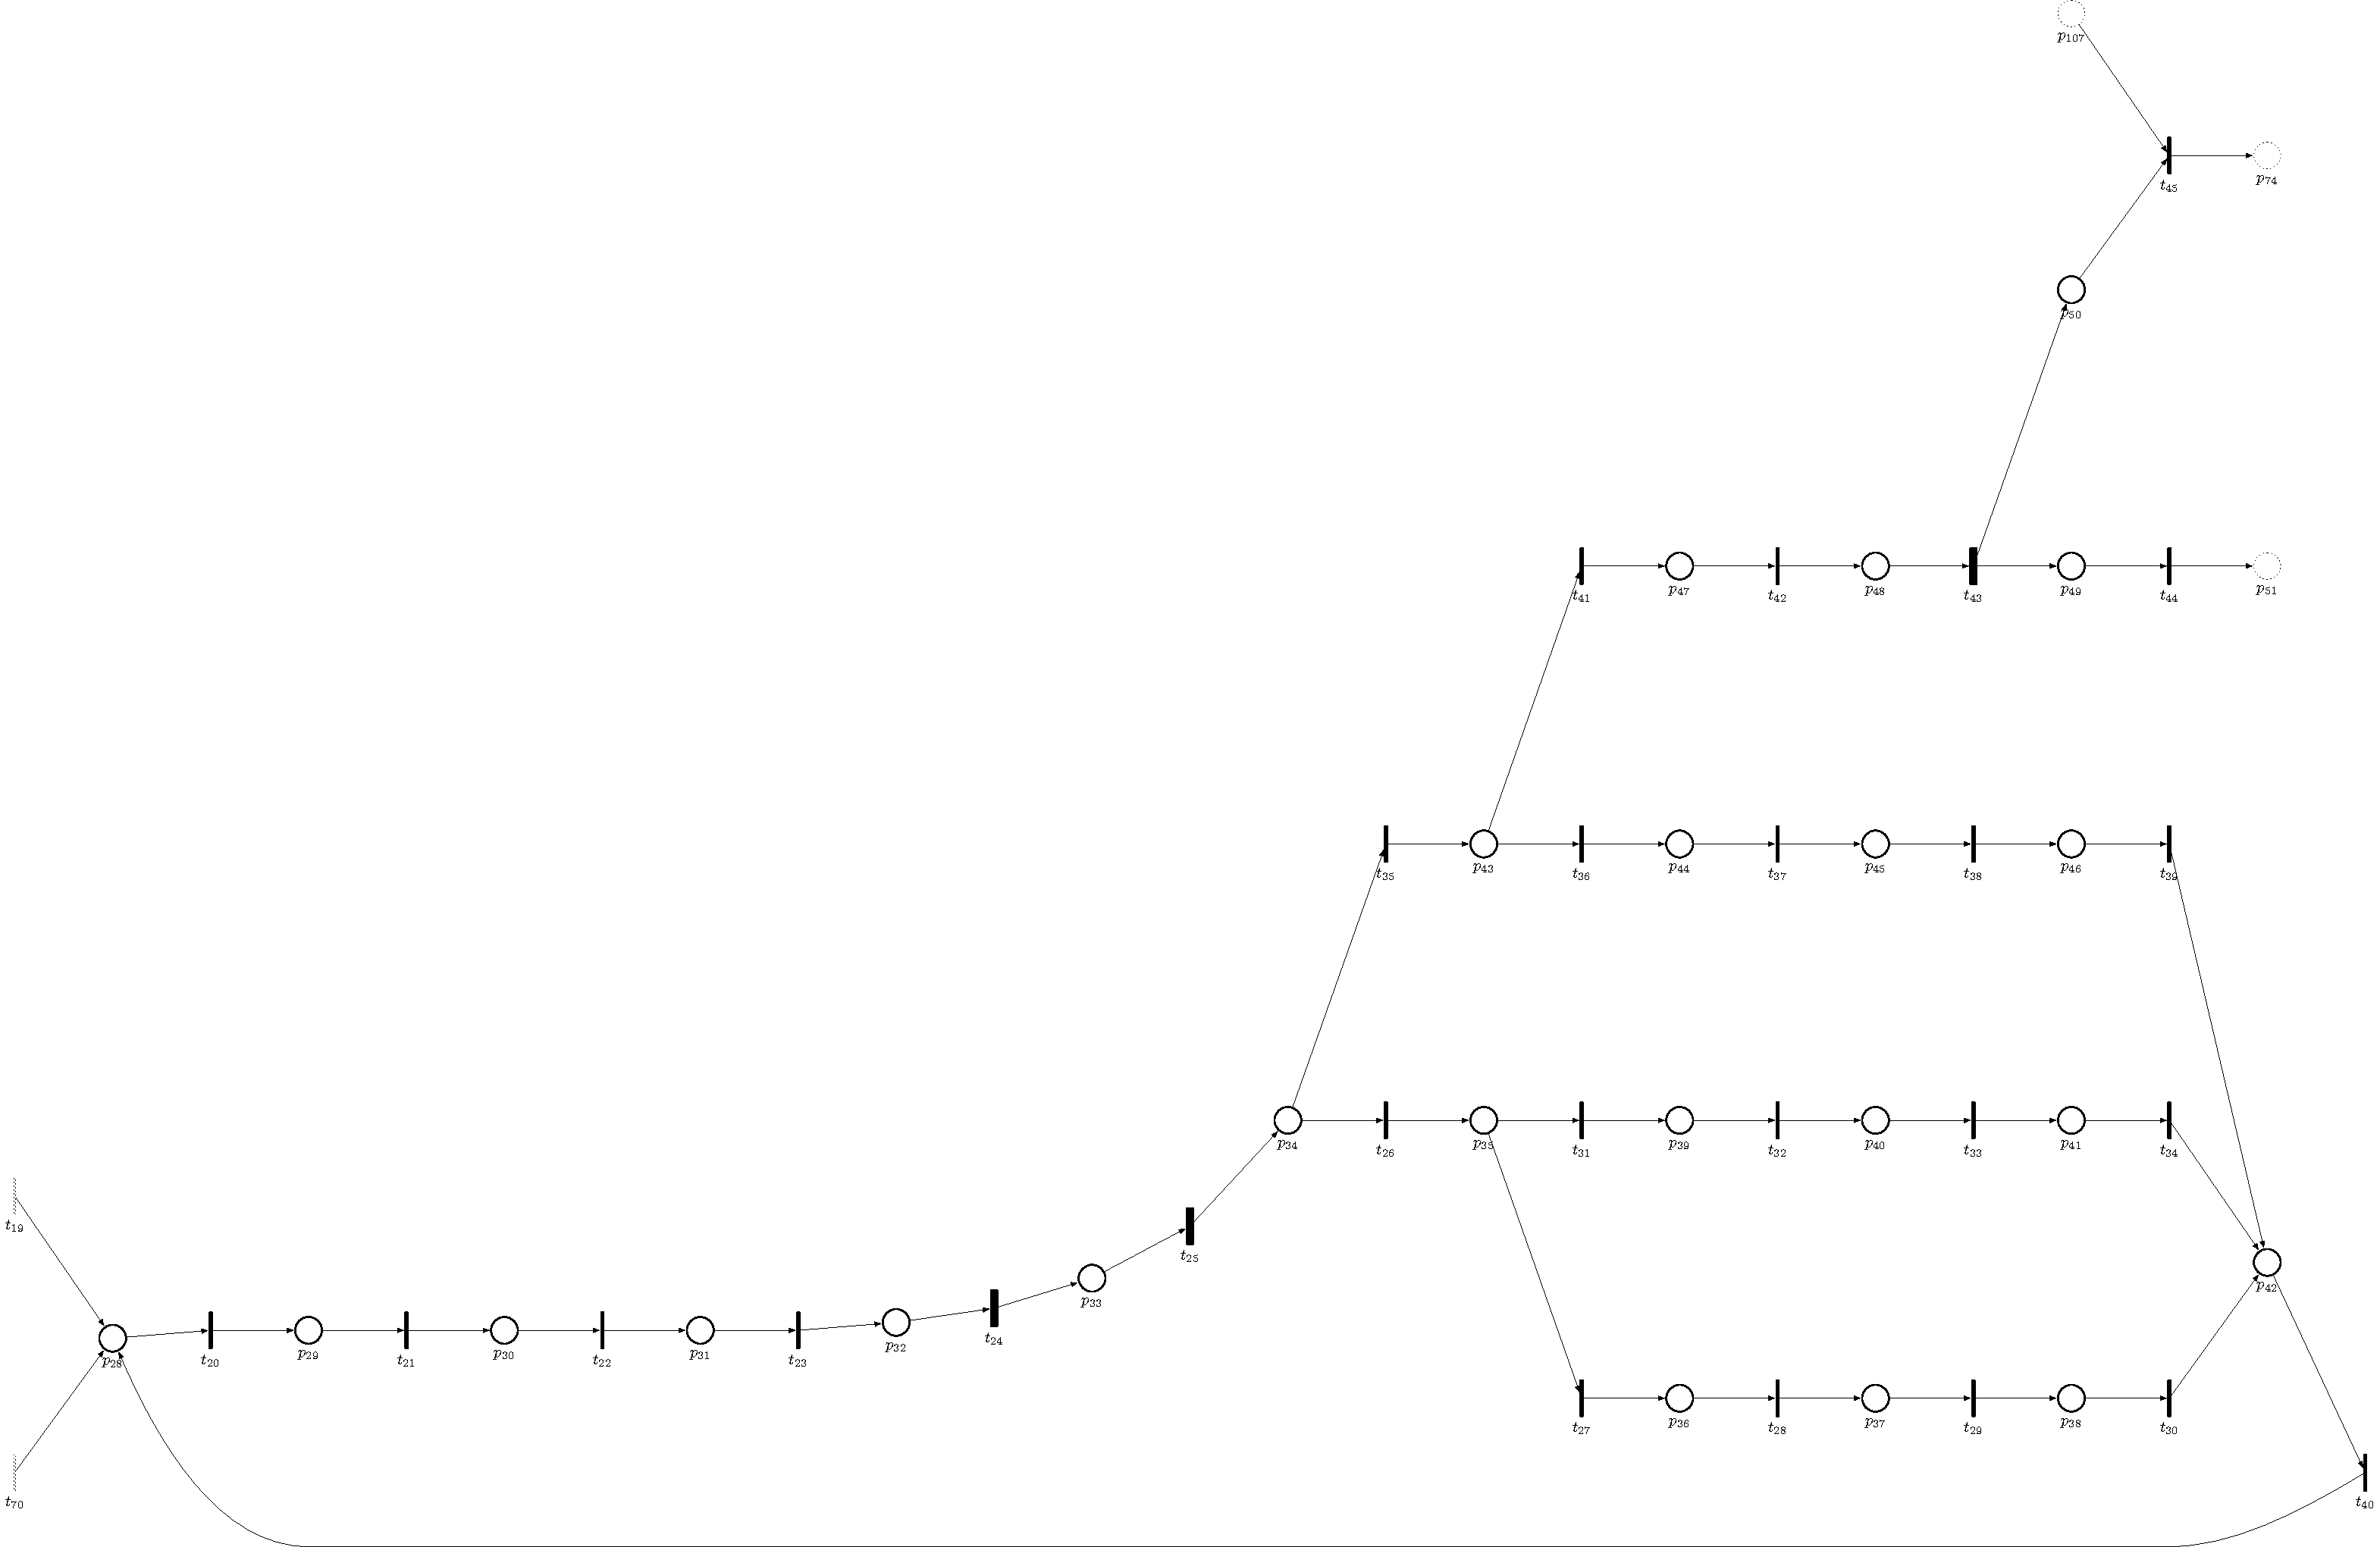
\includegraphics{../../figures/petriNet/dot/2-metalv/metalv.pdf}
%   \caption{qlksdjf}
%   \label{fig:example}
% \end{figure}


% \begin{figure}[H]
%   \centering
%   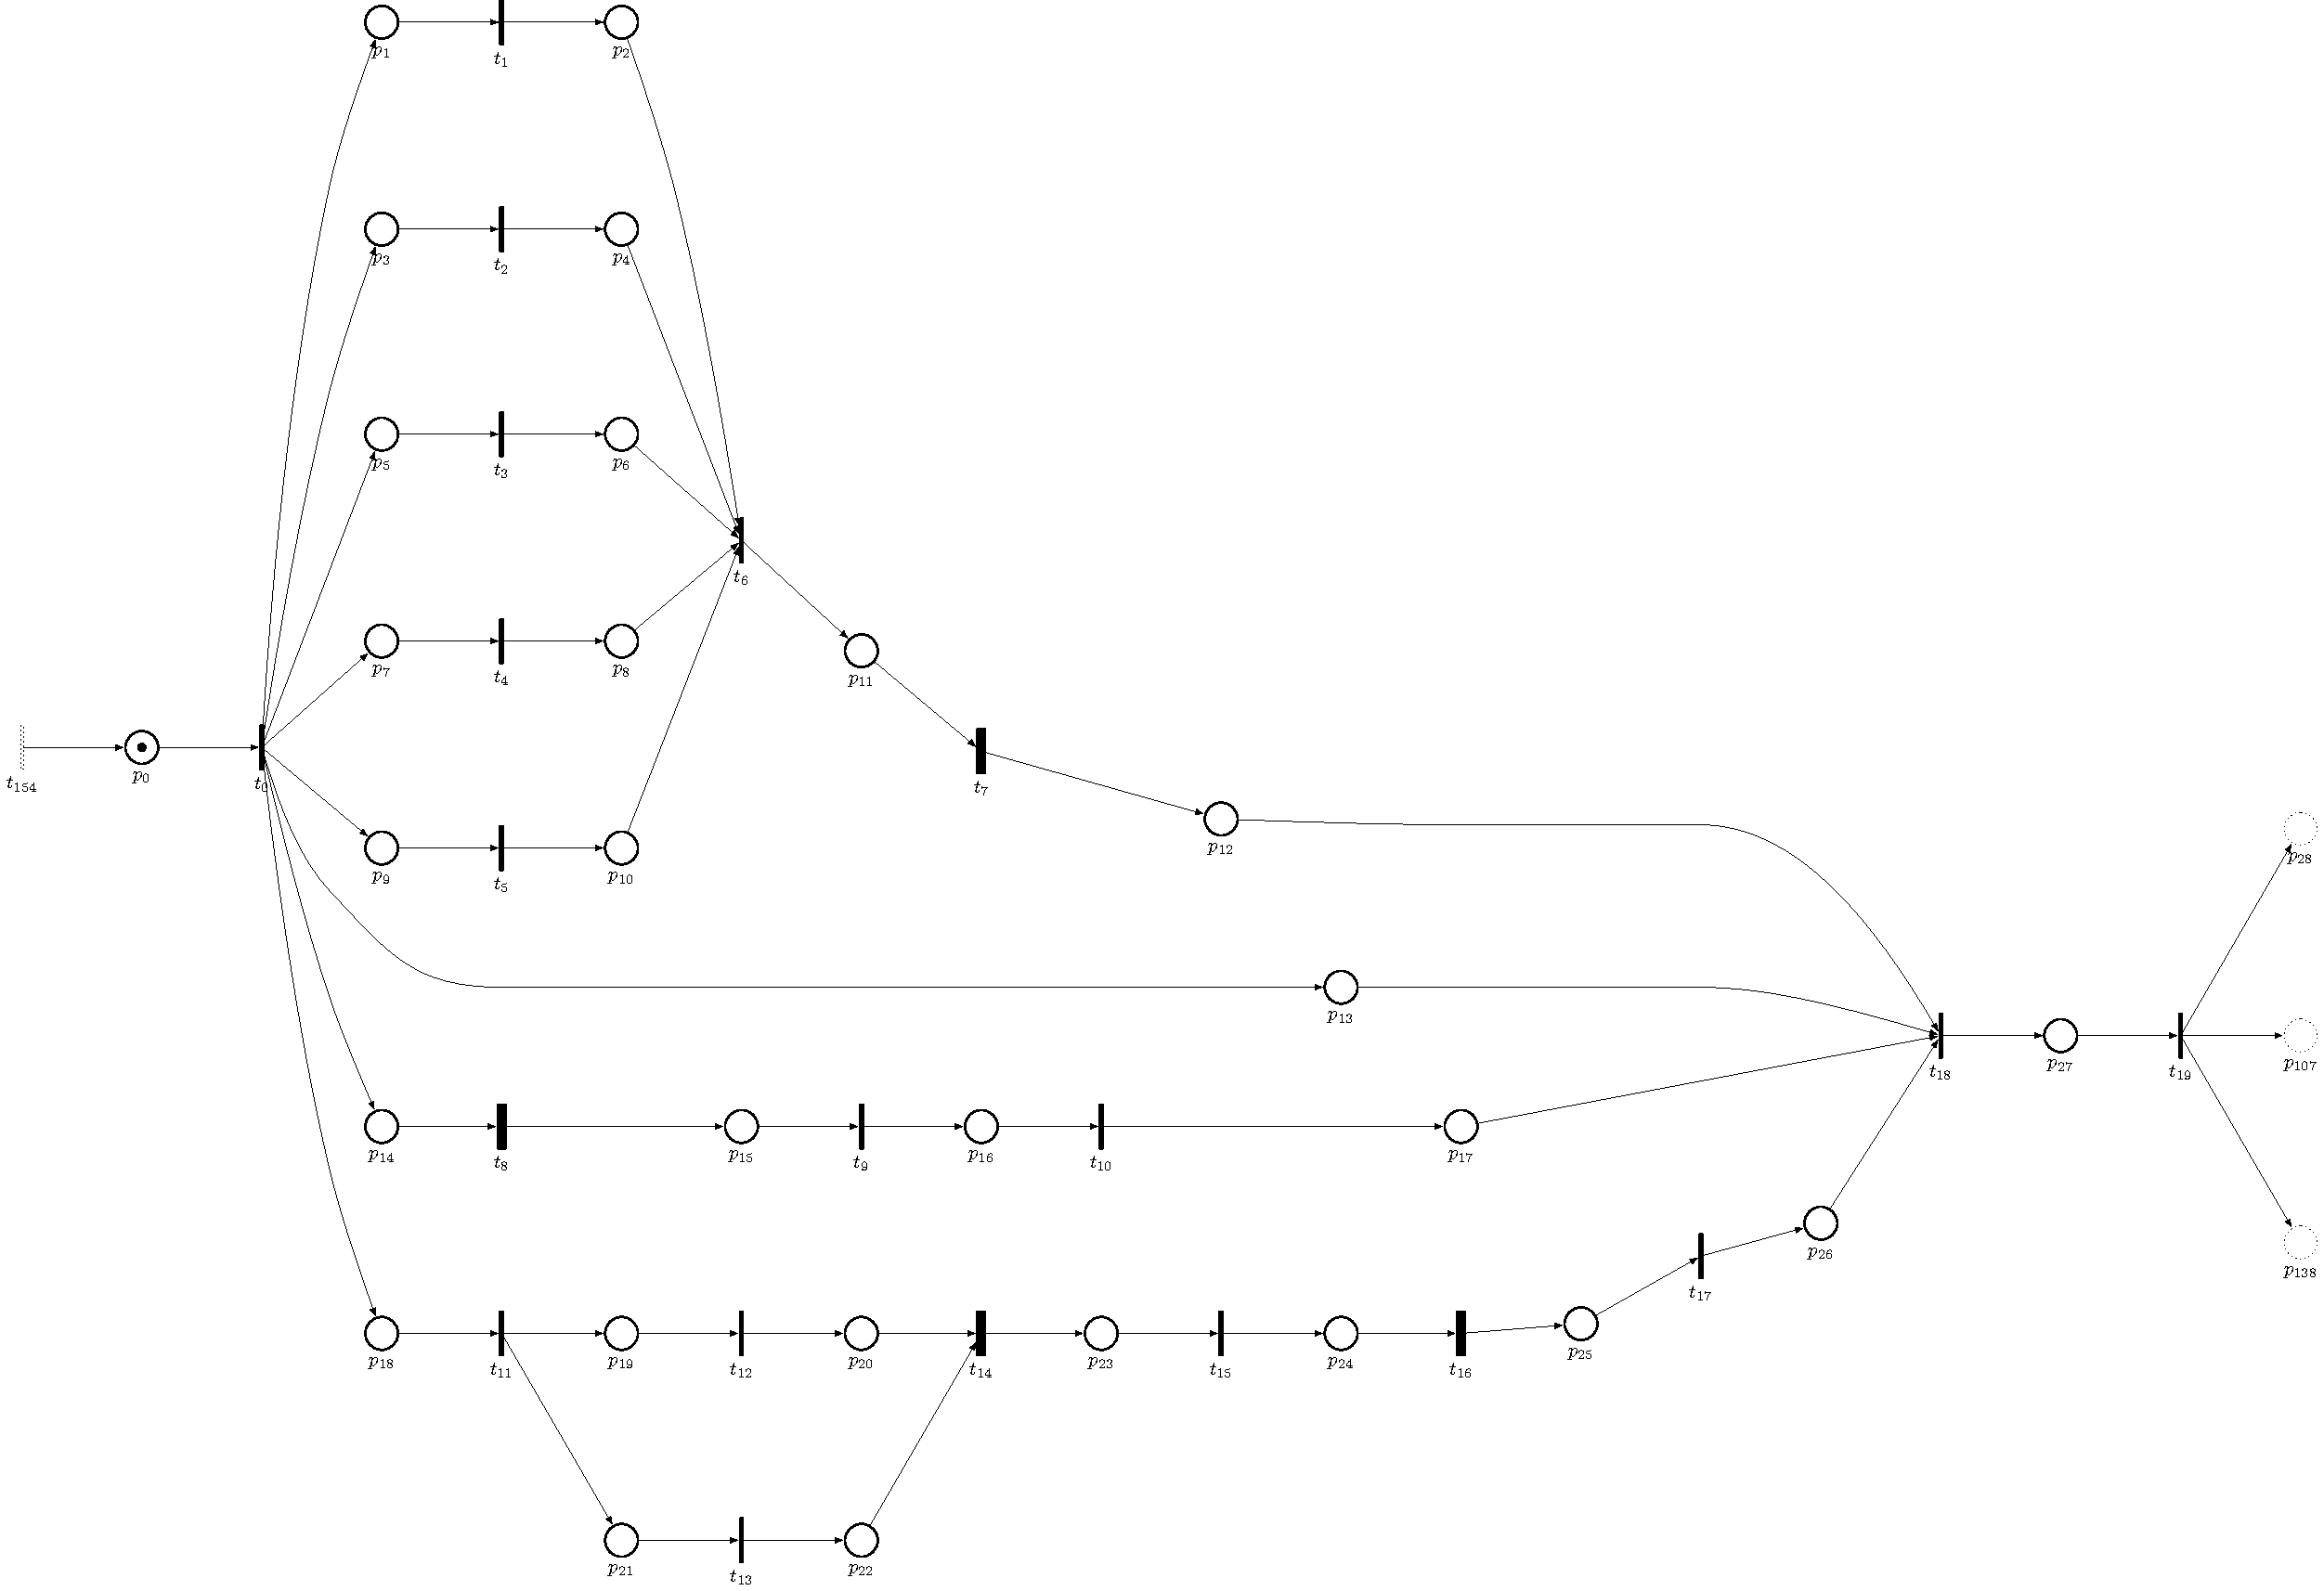
\includegraphics[width=0.4\textwidth]{../../figures/partial/initial.tikz}
%   \caption{petri net bal}
%   \label{fig:petrinetexample}
% \end{figure}

% \addtikzfigure{../../figures/petriNet/partial/initial}
% {Petri net of cube storage module.}
% {petri_initialization}

% \addtikzfigure{../../figures/petriNet//partial/metalv}
% {Petri net of metal cube half sorting module.}
% {petri_initialization}

\begin{table}[htbp]
\caption{Initialization Module Places.}
\centering
\begin{tabular}{M{5cm}M{10cm}}
Places & Meaning\\
\hline
\hyperlink{partialNet:p0m1}{\hypertarget{partialTable:p0m1}{$p_{0}$}} & System Stopped\\
\hyperlink{partialNet:p1}{\hypertarget{partialTable:p1}{$p_{1}$}} & Retract MAG1's Cylinder *\\
\hyperlink{partialNet:p2}{\hypertarget{partialTable:p2}{$p_{2}$}} & MAG1's Cylinder Retracted\\
\hyperlink{partialNet:p3}{\hypertarget{partialTable:p3}{$p_{3}$}} & Retract MAG2's Cylinder *\\
\hyperlink{partialNet:p4}{\hypertarget{partialTable:p4}{$p_{4}$}} & MAG2's Cylinder Retracted\\
\hyperlink{partialNet:p5}{\hypertarget{partialTable:p5}{$p_{5}$}} & Retract Right Discharge Cylinder *\\
\hyperlink{partialNet:p6}{\hypertarget{partialTable:p6}{$p_{6}$}} & Right Discharge Cylinder Retracted\\
\hyperlink{partialNet:p7}{\hypertarget{partialTable:p7}{$p_{7}$}} & Retract Center Discharge Cylinder\\
\hyperlink{partialNet:p8}{\hypertarget{partialTable:p8}{$p_{8}$}} & Center Discharge Cylinder Retracted\\
\hyperlink{partialNet:p9}{\hypertarget{partialTable:p9}{$p_{9}$}} & Retract Left Discharge Cylinder *\\
\hyperlink{partialNet:p10}{\hypertarget{partialTable:p10}{$p_{10}$}} & Left Discharge Cylinder Retracted\\
\hyperlink{partialNet:p11}{\hypertarget{partialTable:p11}{$p_{11}$}} & Turn Conveyor Belt On (Reverse)\\
\hyperlink{partialNet:p12}{\hypertarget{partialTable:p12}{$p_{12}$}} & No Pieces On Conveyor Belt\\
\hyperlink{partialNet:p13}{\hypertarget{partialTable:p13}{$p_{13}$}} & Reset Variables\\
\hyperlink{partialNet:p14}{\hypertarget{partialTable:p14}{$p_{14}$}} & Raise Press\\
\hyperlink{partialNet:p15}{\hypertarget{partialTable:p15}{$p_{15}$}} & Open Safety Door\\
\hyperlink{partialNet:p16}{\hypertarget{partialTable:p16}{$p_{16}$}} & Extend Assembly Unit Holder\\
\hyperlink{partialNet:p17}{\hypertarget{partialTable:p17}{$p_{17}$}} & Assembly Unit Ready\\
\hyperlink{partialNet:p18}{\hypertarget{partialTable:p18}{$p_{18}$}} & Arm Lowered and Retracted, and Storage Unit Retracted\\
\hyperlink{partialNet:p19}{\hypertarget{partialTable:p19}{$p_{19}$}} & Move Storage Unit to the Right\\
\hyperlink{partialNet:p20}{\hypertarget{partialTable:p20}{$p_{20}$}} & Storage Unit ready ( horizontal )\\
\hyperlink{partialNet:p21}{\hypertarget{partialTable:p21}{$p_{21}$}} & Move Storage Device Downwards\\
\hyperlink{partialNet:p22}{\hypertarget{partialTable:p22}{$p_{22}$}} & Storage Unit ready ( vertical )\\
\hyperlink{partialNet:p23}{\hypertarget{partialTable:p23}{$p_{23}$}} & Rotate Arm CCW\\
\hyperlink{partialNet:p24}{\hypertarget{partialTable:p24}{$p_{24}$}} & Turn HSC Off ( Arm Stopped )\\
\hyperlink{partialNet:p25}{\hypertarget{partialTable:p25}{$p_{25}$}} & Rotate Arm CW\\
\hyperlink{partialNet:p26}{\hypertarget{partialTable:p26}{$p_{26}$}} & Arm Stopped facing conveyor belt\\
\hyperlink{partialNet:p27}{\hypertarget{partialTable:p27}{$p_{27}$}} & System Ready\\
\end{tabular}
\end{table}


\begin{table}[H]
\caption{Initialization Module Transitions.}
\centering
\begin{tabular}{M{5cm}M{10cm}}
Transitions & Meaning\\
\hline
\hyperlink{partialNet:t0}{\hypertarget{partialTable:t0}{$t_{0}$}} & Initialization Button\\
\hyperlink{partialNet:t1}{\hypertarget{partialTable:t1}{$t_{1}$}} & MAG1's Cylinder Retracted\\
\hyperlink{partialNet:t2}{\hypertarget{partialTable:t2}{$t_{2}$}} & MAG2's Cylinder Retracted\\
\hyperlink{partialNet:t3}{\hypertarget{partialTable:t3}{$t_{3}$}} & Right Discharge Cylinder Retracted\\
\hyperlink{partialNet:t4}{\hypertarget{partialTable:t4}{$t_{4}$}} & Center Discharge Cylinder Retracted\\
\hyperlink{partialNet:t5}{\hypertarget{partialTable:t5}{$t_{5}$}} & Left Discharge Cylinder Retracted\\
\hyperlink{partialNet:t6}{\hypertarget{partialTable:t6}{$t_{6}$}} & \\
\hyperlink{partialNet:tt7}{\hypertarget{partialTable:tt7}{$t_{7}$}} & T=12s\\
\hyperlink{partialNet:tt8}{\hypertarget{partialTable:tt8}{$t_{8}$}} & T=2.5s\\
\hyperlink{partialNet:t9}{\hypertarget{partialTable:t9}{$t_{9}$}} & Safety Door Opened\\
\hyperlink{partialNet:t10}{\hypertarget{partialTable:t10}{$t_{10}$}} & Assembly Unit Holder Extended\\
\hyperlink{partialNet:t11}{\hypertarget{partialTable:t11}{$t_{11}$}} & Storage Unit Retracted and Arm Lowered and Retracted\\
\hyperlink{partialNet:t12}{\hypertarget{partialTable:t12}{$t_{12}$}} & Storage Unit Right Limit Switch\\
\hyperlink{partialNet:t13}{\hypertarget{partialTable:t13}{$t_{13}$}} & Storage Unit Inferior Limit Switch\\
\hyperlink{partialNet:tt14}{\hypertarget{partialTable:tt14}{$t_{14}$}} & T=2s\\
\hyperlink{partialNet:t15}{\hypertarget{partialTable:t15}{$t_{15}$}} & Inductive Sensor Arm\\
\hyperlink{partialNet:tt16}{\hypertarget{partialTable:tt16}{$t_{16}$}} & T=1s\\
\hyperlink{partialNet:t17}{\hypertarget{partialTable:t17}{$t_{17}$}} & ARMCOUNTER <= BELT\_ANGLE\_CW\\
\hyperlink{partialNet:t18}{\hypertarget{partialTable:t18}{$t_{18}$}} & \\
\hyperlink{partialNet:t19}{\hypertarget{partialTable:t19}{$t_{19}$}} & Start Button\\
\end{tabular}
\end{table}


\begin{longtable}{M{5cm}M{10cm}}
\caption{Metal Half-cube Selection Module Places.} \label{tab:metalvPlaces}
\\
Places & Meaning\\
\hline
\endfirsthead
\multicolumn{2}{l}{Continued from previous page} \\
\hline

Places & Meaning \\

\hline
\endhead
\hline\multicolumn{2}{r}{Continued on next page} \\
\endfoot
\endlastfoot
\hline
\hyperlink{partialNet:p28}{\hypertarget{partialTable:p28}{$p_{28}$}} & MAG1 Empty\\
\hyperlink{partialNet:p29}{\hypertarget{partialTable:p29}{$p_{29}$}} & MAG1 Not Empty\\
\hyperlink{partialNet:p30}{\hypertarget{partialTable:p30}{$p_{30}$}} & Extend MAG1's Cylinder *\\
\hyperlink{partialNet:p31}{\hypertarget{partialTable:p31}{$p_{31}$}} & Retract MAG1's Cylinder *\\
\hyperlink{partialNet:p32}{\hypertarget{partialTable:p32}{$p_{32}$}} & MAG1's Cylinder Retracted\\
\hyperlink{partialNet:p33}{\hypertarget{partialTable:p33}{$p_{33}$}} & Turn Conveyor Belt On\\
\hyperlink{partialNet:p34}{\hypertarget{partialTable:p34}{$p_{34}$}} & \\
\hyperlink{partialNet:p35}{\hypertarget{partialTable:p35}{$p_{35}$}} & Plastic Half-cube\\
\hyperlink{partialNet:p36}{\hypertarget{partialTable:p36}{$p_{36}$}} & Turn Conveyor Belt On\\
\hyperlink{partialNet:p37}{\hypertarget{partialTable:p37}{$p_{37}$}} & Extend Right Discharge Cylinder *\\
\hyperlink{partialNet:p38}{\hypertarget{partialTable:p38}{$p_{38}$}} & Retract Right Discharge Cylinder *\\
\hyperlink{partialNet:p39}{\hypertarget{partialTable:p39}{$p_{39}$}} & Turn Conveyor Belt On\\
\hyperlink{partialNet:p40}{\hypertarget{partialTable:p40}{$p_{40}$}} & Extend Center Discharge Cylinder *\\
\hyperlink{partialNet:p41}{\hypertarget{partialTable:p41}{$p_{41}$}} & Retract Center Discharge Cylinder *\\
\hyperlink{partialNet:p42}{\hypertarget{partialTable:p42}{$p_{42}$}} & \\
\hyperlink{partialNet:p43}{\hypertarget{partialTable:p43}{$p_{43}$}} & Metal Half-cube\\
\hyperlink{partialNet:p44}{\hypertarget{partialTable:p44}{$p_{44}$}} & Turn Conveyor Belt On\\
\hyperlink{partialNet:p45}{\hypertarget{partialTable:p45}{$p_{45}$}} & Extend Left Discharge Cylinder *\\
\hyperlink{partialNet:p46}{\hypertarget{partialTable:p46}{$p_{46}$}} & Retract Left Discharge Cylinder *\\
\hyperlink{partialNet:p47}{\hypertarget{partialTable:p47}{$p_{47}$}} & Turn Conveyor Belt On\\
\hyperlink{partialNet:p48}{\hypertarget{partialTable:p48}{$p_{48}$}} & Turn Conveyor Belt On\\
\hyperlink{partialNet:p49}{\hypertarget{partialTable:p49}{$p_{49}$}} & Metal Half-cube Ready\\
\hyperlink{partialNet:p50}{\hypertarget{partialTable:p50}{$p_{50}$}} & Conveyor Belt Stopped\\
\end{longtable}


\begin{table}[H]
\caption{Metal Half-cube Selection Module Transitions.}
\centering
\begin{tabular}{M{5cm}M{10cm}}
Transitions & Meaning\\
\hline
\hyperlink{partialNet:t20}{\hypertarget{partialTable:t20}{$t_{20}$}} & \(\overline{\mbox{MAG1 Empty}}\)\\
\hyperlink{partialNet:t21}{\hypertarget{partialTable:t21}{$t_{21}$}} & \\
\hyperlink{partialNet:t22}{\hypertarget{partialTable:t22}{$t_{22}$}} & MAG1's Cylinder Extended \(\uparrow\)\\
\hyperlink{partialNet:t23}{\hypertarget{partialTable:t23}{$t_{23}$}} & MAG1's Cylinder Retracted \(\uparrow\)\\
\hyperlink{partialNet:tt24}{\hypertarget{partialTable:tt24}{$t_{24}$}} & T=0.5s\\
\hyperlink{partialNet:tt25}{\hypertarget{partialTable:tt25}{$t_{25}$}} & Presence \(\uparrow\) T=0.5s\\
\hyperlink{partialNet:t26}{\hypertarget{partialTable:t26}{$t_{26}$}} & \(\overline{\mbox{Metallic Sensor}}\)\\
\hyperlink{partialNet:t27}{\hypertarget{partialTable:t27}{$t_{27}$}} & \(\overline{\mbox{White Color Sensor}}\)\\
\hyperlink{partialNet:t28}{\hypertarget{partialTable:t28}{$t_{28}$}} & Proximity Sensor Left Discharge Cylinder \(\uparrow\)\\
\hyperlink{partialNet:t29}{\hypertarget{partialTable:t29}{$t_{29}$}} & Right Discharge Cylinder Extended\\
\hyperlink{partialNet:t30}{\hypertarget{partialTable:t30}{$t_{30}$}} & Right Discharge Cylinder Retracted\\
\hyperlink{partialNet:t31}{\hypertarget{partialTable:t31}{$t_{31}$}} & White Color Sensor\\
\hyperlink{partialNet:t32}{\hypertarget{partialTable:t32}{$t_{32}$}} & Proximity Sensor Center Discharge Cylinder \(\uparrow\)\\
\hyperlink{partialNet:t33}{\hypertarget{partialTable:t33}{$t_{33}$}} & Center Discharge Cylinder Extended\\
\hyperlink{partialNet:t34}{\hypertarget{partialTable:t34}{$t_{34}$}} & Center Discharge Cylinder Retracted\\
\hyperlink{partialNet:t35}{\hypertarget{partialTable:t35}{$t_{35}$}} & Metallic Sensor\\
\hyperlink{partialNet:t36}{\hypertarget{partialTable:t36}{$t_{36}$}} & Concavity Downwards\\
\hyperlink{partialNet:t37}{\hypertarget{partialTable:t37}{$t_{37}$}} & Proximity Sensor Left Discharge Cylinder \(\uparrow\)\\
\hyperlink{partialNet:t38}{\hypertarget{partialTable:t38}{$t_{38}$}} & Left Discharge Cylinder Extended\\
\hyperlink{partialNet:t39}{\hypertarget{partialTable:t39}{$t_{39}$}} & Left Discharge Cylinder Retracted\\
\hyperlink{partialNet:t40}{\hypertarget{partialTable:t40}{$t_{40}$}} & \\
\hyperlink{partialNet:t41}{\hypertarget{partialTable:t41}{$t_{41}$}} & Concavity Upwards\\
\hyperlink{partialNet:t42}{\hypertarget{partialTable:t42}{$t_{42}$}} & Proximity Sensor End Of Conveyor Belt \(\uparrow\)\\
\hyperlink{partialNet:tt43}{\hypertarget{partialTable:tt43}{$t_{43}$}} & T=0.5s\\
\hyperlink{partialNet:t44}{\hypertarget{partialTable:t44}{$t_{44}$}} & Proximity Sensor End Of Conveyor Belt \(\downarrow\)\\
\hyperlink{partialNet:t45}{\hypertarget{partialTable:t45}{$t_{45}$}} & \\
\end{tabular}
\end{table}


%%% Local Variables:
%%% mode: latex
%%% TeX-master: "../monografia"
%%% End:



\chapter{Introduction}
In a world where the majority of the population lives in industrial societies,
and machines take part on the bulk of the production of almost all goods: from
food to cosmetics and drugs, from toothbrushes to automobiles, 
a well-paced throughput it is crucial, and any non expected halt on the
production or change can be disastrous, producing sometimes multimillionaire debts,
provoking a snowball effect, affecting the economy and consequentially the welfare of the society.

A diverse number of causes of the halt or change of the throughput can be
accounted for. Some are as simple as a power outage, or a component malfunction,
but nowadays there are other players. As the industry \textsl{walks}, or even
better \textsl{runs}, towards the so called Fourth Industrial Revolution, the industry
urges the use of \textit{connected sensors}, since the Internet of Things is the
fashion these days, but the concerns about cyber security are now and again neglected.   
So hackers can infiltrate the system, and depending of the infrastructure
halt or change somehow the production throughput.

Cyber security is not the theme of this thesis but its theme is another important concern to a
well-paced throughput, failure detection.

As great part of the manufacture facilities uses conveyor
belts, pneumatic cylinders and digital sensors, it is very common to see \PLCs



\PLC 




\acr{oi}{oi}{oi}
\oi





khe  the most simple as  In order to prevent these effects lots of 
\todo{ objetivo mostrar que o metodo pode funcionar 
com comportamento paraelo mostrar a escabilidade
}
\doing{the objective of this thesis is to show that the \DAOCT model works with
  systems that presents parallel behavior dividing themand can be used to scalability }
\section{Thesis Outline}
\label{sec:thesisOutline}






%%% Local Variables:
%%% mode: latex
%%% TeX-master: "../monografia.tex"
%%% End:

\chapter{Results}
\label{cha:results}

In this 2 paths
best 80 paths States
all
1321  2166  2962  3744  4508  5235  5939

best
1294  2127  2904  3663  4395  5088  5746
\begin{figure}[H]
  \centering
  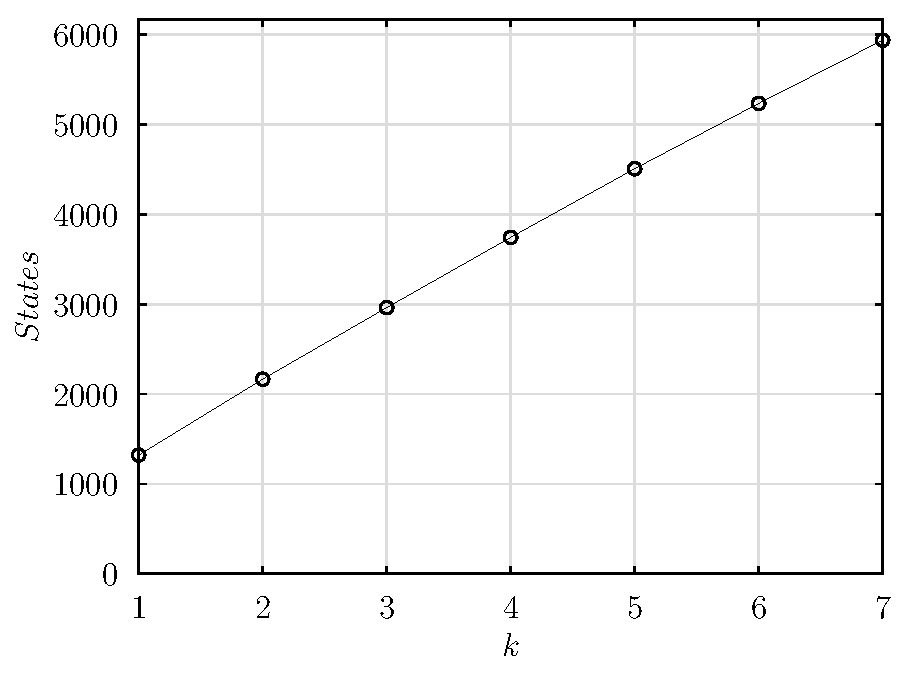
\includegraphics[width=0.5\textwidth]{results/all/states.pdf}
  \caption{Input\slash Output Process model}
    \label{fig:ioProcModel}
\end{figure}
\begin{figure}[H]
  \centering
  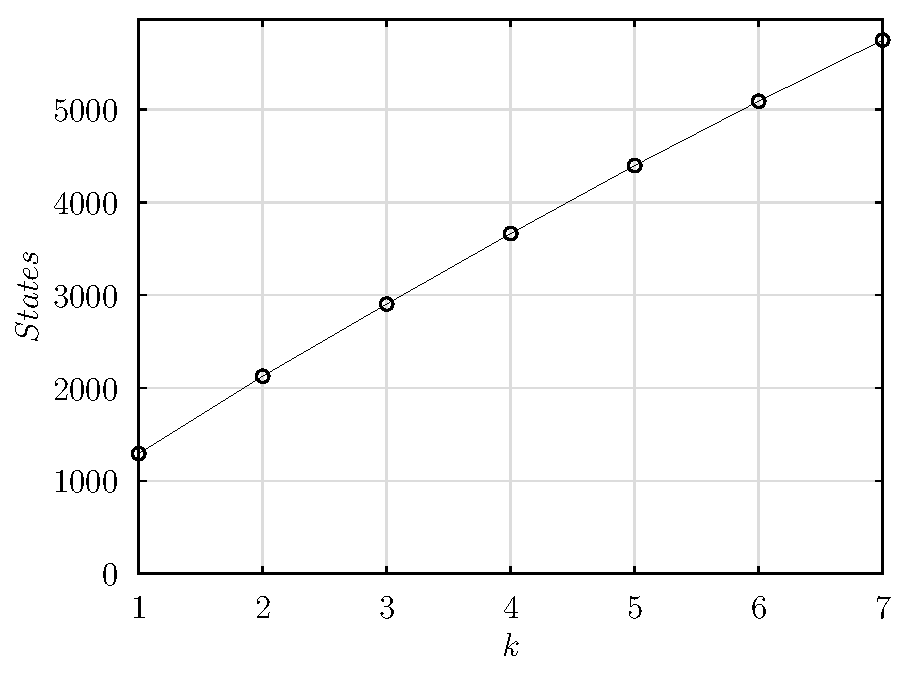
\includegraphics[width=0.5\textwidth]{results/all/best/states.pdf}
  \caption{Input\slash Output Process model}
    \label{fig:ioProcModel}
\end{figure}
\begin{figure}[H]
  \centering
  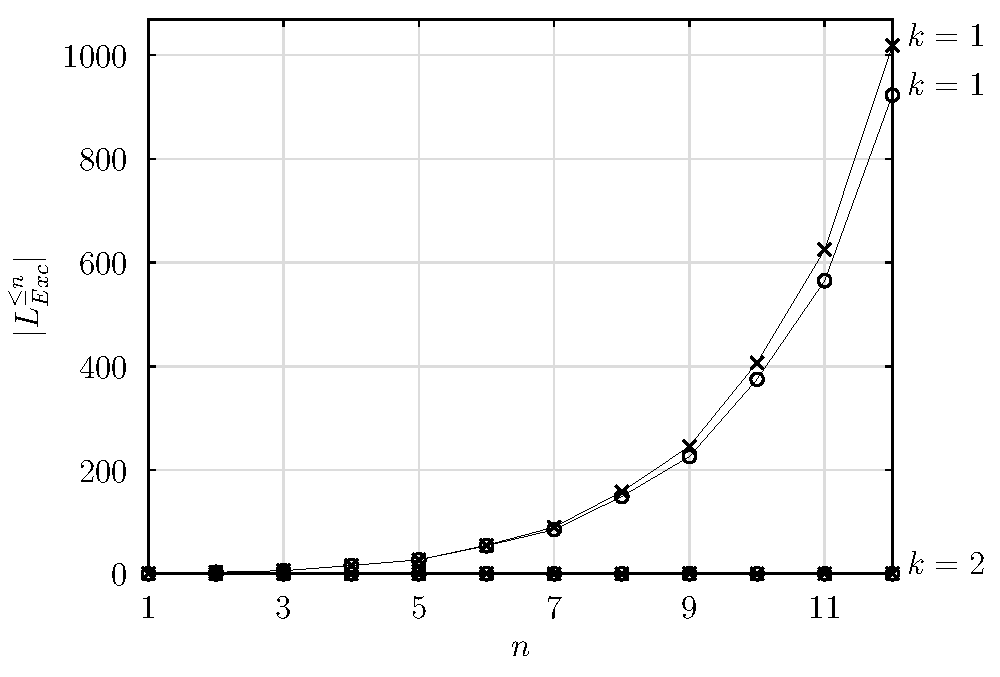
\includegraphics[width=0.5\textwidth]{results/all/exceedingLanguage-daoct-ndaao_k1-2_n12.pdf}
  \caption{Input\slash Output Process model}
    \label{fig:ioProcModel}
\end{figure}

 \section{best} 
\begin{figure}[H]
\begin{subfigure}[H]{0.5\textwidth}
  \centering
  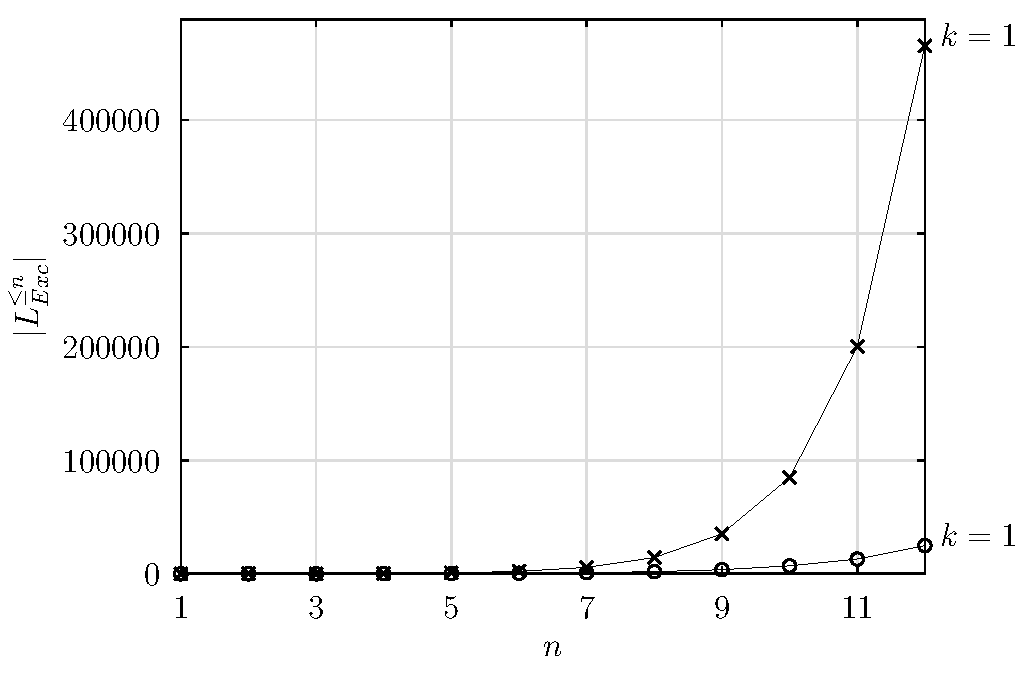
\includegraphics[width=\textwidth]{results/all/best/exceedingLanguage-daoct-ndaao_k1_n12.pdf}
  \caption{Input\slash Output Process model}
    \label{fig:ioProcModel}
\end{subfigure}
\begin{subfigure}[h]{0.5\textwidth}
  \centering
  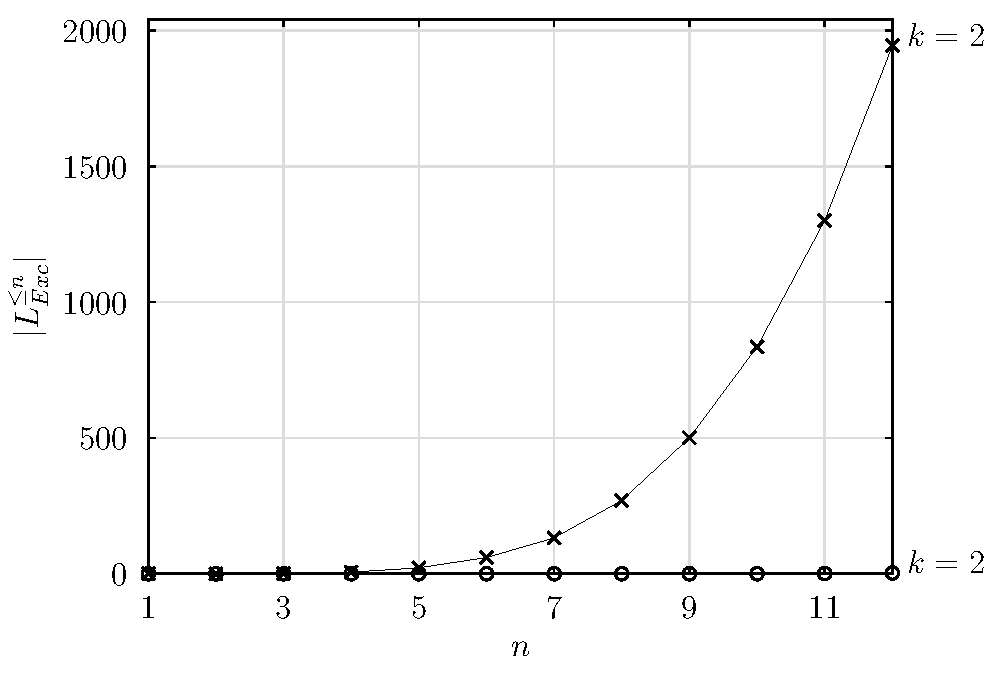
\includegraphics[width=\textwidth]{results/all/best/exceedingLanguage-daoct-ndaao_k2_n12.pdf}
  \caption{Input\slash Output Process model}
    \label{fig:ioProcModel}
\end{subfigure}
\end{figure}
\section{DAOCT}
\label{sec:results_daoct}

\section{Discussion about the identification}
\begin{figure}[H]
  \centering
  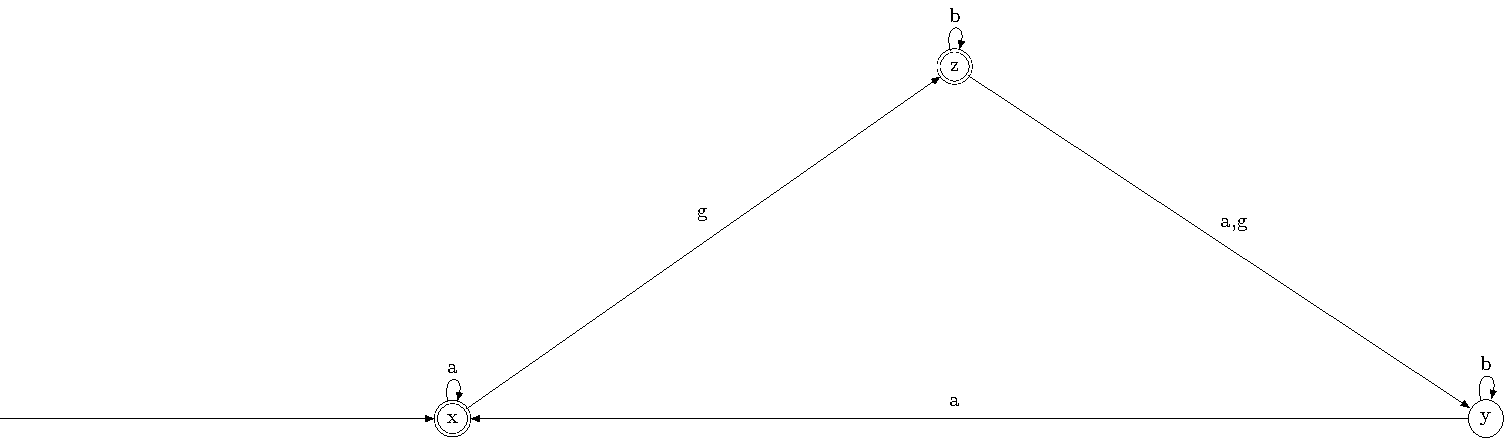
\includegraphics{results/example/example}
  \caption{Input\slash Output Process model}
    \label{fig:ioProcModel}
\end{figure}


\begin{figure}[H]
  \centering
  \includegraphics{results/example/examplek1NoArrows}
  \caption{Input\slash Output Process model}
    \label{fig:ioProcModel}
\end{figure}

\begin{figure}[H]
  \centering
  \includegraphics{results/example/example1k1NoArrows}
  \caption{Input\slash Output Process model}
    \label{fig:ioProcModel}
\end{figure}

\begin{figure}[H]
  \centering
  \includegraphics{results/example/example1k2NoArrows}
  \caption{Input\slash Output Process model}
    \label{fig:ioProcModel}
\end{figure}
% \begin{figure}[H]
%   \centering
%   \includegraphics[width=0.5\textwidth]{exceedingLanguage/example/exceedingLanguage-daoct-ndaao_k2_n7.pdf}
%   \caption{Cardinality of the exceeding language of the DAOCT (o) and NDAAO
%     ($\times$) models. $k = 1$, and $1 \leq n \leq 7$}
%   \label{fig:exceedingLangExample}
% \end{figure}


% Comparing the results of the \autoref{fig:exceedingLangExample}  with the
% example 3 from \cite{moreira2018enhanced}, we can
% observe that the exceeding language for the DAOCT model drops. This is caused by
% how the acquisition works, in this work, the plant is considered a black box, so
% instead of feeding the algorithm with the
% paths, the raw data is given, and the paths are calculated using the first
% IO\_Vector as the initial state and once this initial state is repeated other
% path 
% is created, resulting on 4 paths instead of 3. This change, can result in a
% smaller path, with no loops, diminishing the exceeding language.


% \section{Manufacture System}
% \label{sec:results_system}

% \begin{figure}[H]
%   \centering
%   \includegraphics[width=0.5\textwidth]{results/all/exceedingLanguage-daoct-ndaao_k1_n7.pdf}
%   \caption{graph}
% \end{figure}

% \begin{figure}[H]
%   \centering
%   \includegraphics[width=0.5\textwidth]{results/all/exceedingLanguage-daoct-ndaao_k2-3-7_n25.pdf}
%   \caption{graph}
% \end{figure}

% \todo{Choosing the IO\_Vector with the greatest repetition ratio as $x_0$}

% \begin{figure}[H]
%   \centering
%   \includegraphics[width=0.5\textwidth]{results/all/best/exceedingLanguage-daoct-ndaao_k1_n7.pdf}
%   \caption{graph}
% \end{figure}


% \begin{figure}[H]
%   \centering
%   \includegraphics[width=0.5\textwidth]{results/all/best/exceedingLanguage-daoct-ndaao_k2-3-7_n25.pdf}
%   \caption{graph}
% \end{figure}

% Removing I\_MAG1EMPT and I\_MAG2EMPT

% \begin{figure}[H]
%   \centering
%   \includegraphics[width=0.5\textwidth]{results/all-2_5/exceedingLanguage-daoct-ndaao_k1_n7.pdf}
%   \caption{graph}
% \end{figure}

% \todo{Choosing the IO\_Vector with the greatest repetition ratio as $x_0$}

% \begin{figure}[H]
%   \centering
%   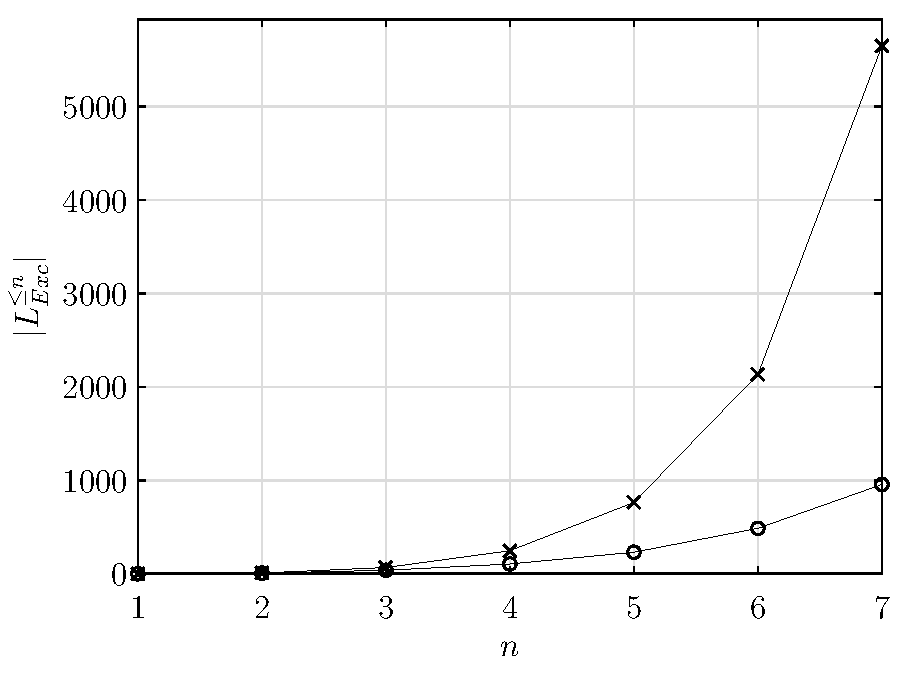
\includegraphics[width=0.5\textwidth]{results/all-2_5/best/exceedingLanguage-daoct-ndaao_k1_n7.pdf}
%   \caption{graph}
% \end{figure}

% As we can see, the exceedingLanguage raises




%%% Local Variables:
%%% mode: latex
%%% TeX-master: "../monografia"
%%% End:

\chapter{Conclusion}
\label{cha:conclusion}
% As proposed in the introduction, this work presents a methodology and tools for
% control, observation and identification of \DESs{} in order to have a model to be
% used for fault detection. In this chapter a brief retrospective of the process
% of preparation of the methodology and the tools presented is made. And then the
% conclusions are drawn based on the results generated by the application of
% the methodology
% to identify a didactic manufacturing system.
% The control implementation was based on the
% method shown in \cite{moreira2013bridging} and the identification model based on \cite{moreira2018enhanced}.
% This identification method based on the
% observation of the fault-free behaviour of the system
% acquisition , from its conception.

% Through the process of preparation of the methodology and tools, some issues
% were found, and they are compiled in this chapter. Some
% workarounds are proposed as new approaches to solve these issues in future works.

\section{Concluding Remarks}
\label{sec:concludingRemarks}
In this work a method for the control, observation and identification of a
\DES{} was presented. First, the control logic was created using a \CIPN, and then implemented
in \LD{} to be used in a Siemens \PLC{} (\Autoref{cha:control}). After that, the observation of the
inputs and outputs of the controller was made using data log function blocks that saved the data in
\verb|.csv| files, and finally, these \verb|.csv| files were used as the input of the
identification algorithm generating a \DAOCT{} model (\Autoref{cha:ident}). In
\Autoref{cha:results} we could see that if the system was observed for a long
time and the initial state of observation was well-chosen, then the \DAOCT{} is
a good candidate for modelling, if the aim of this modelling is fault-detection.
The fact that the exceeding language of the \DAOCT{} model drops to $0$ more
rapidly than other models, with a smaller value of the variable $k$, proves that it is less resource intensive than the
others, even for relatively big
systems, with more than $60$ inputs\slash outputs with concurrent behaviour.


\section{Further Work}
An issue found in the implementation of the control is the use of \LD{} to
program the logic. Although \LD{} is very used
in the industry, as it is a visual language, it creates a difficulty for the
automation of the conversion from Petri net. An approach that can be used in
future works would be to represent the Petri net in a text format, Petri net
markup language for instance (presented in \cite{weber2003petri}), and create a
tool that automatically converts this file to a text based language standardised
by the IEC 61131-1, \IL{} or \ST{}. Since \IL{} is less used, \ST{}
would be a better choice. Using a text based language increases portability
of the code and it helps the development, since version control can be used in
text files, allowing the collaboration of multiple people to edit the code if
needed, and track who made the changes, increasing the maintainability
of the code.



Another issue was about the observation. Although the acquisition of
inputs\slash outputs using data logs and saving the data in batches on
\verb|.csv| files can be used for the identification process, for
fault-detection it is not optimal to use this approach, a better one would be to
acquire the data in real time, by using some API, snap7 for example, or using
\SCADA{} protocols.
% But if we use in a future work the function block created to log
% the data in \Autoref{cha:ident}, the \emph{LOGDATA} block, it is recommended to
% optimise its contents. Some refactoring on the logic could be made, increasing its
% speed and removing some unnecessary variables that may be present.

As shown in \Autoref{cha:results}, the didactic manufacturing system used for the
experiments have a considerable concurrent behaviour, affecting the identified
model, on the number of states and extracted paths. As future work would be to divide the observation of the system in its modules, and
compare the multiple models generated by the identification algorithm with the
one using the observation of the complete system.

Another issue shown in \Autoref{cha:results}, is the choice of the first
vector to be used as initial state in the identification algorithm. Here we
propose for future works a study on how to find the optimal vector. Two
scenarios could be considered: the first one taking a grey box approach, where some behaviour
is previously known, by a simple description of the function of the system and another considering a black box approach.

Another proposition for a future work is made in \Autoref{cha:results}. Instead
of using an identification model based on the observation of inputs\slash
outputs of the system, an alternative would be to create and use a model that uses the observation of
the events of the system.


% to extract the paths and events of the system and to identify the system
% behaviour,
% a way out would be to observe the events and use them to identify the
% system. Of course the \DAOCT{} model would not be fit for it, and another model
% should be developed. This way, probably the problem with the choice of the
% initial state of the system would cease to exist.


%%% Local Variables:
%%% mode: latex
%%% TeX-master: "../monografia"
%%% End:


\backmatter

\bibliographystyle{coppe-unsrt}
\nocite{*}
\bibliography{bibliography}

\appendix
\include{appendices/petriNet}
\tikzset{
  place/.style={
    circle,
    thick,
    draw=black!100, % draw=blue!75,
    % fill=blue!20,
    minimum size=0.3mm
  },
  transition/.style={
    rectangle,
    thick,
    fill=black,
    minimum width=2mm,
    inner ysep=0.7pt,
  },
  timedtransition/.style={
    rectangle,
    thick,
    fill=black,
    minimum width=4mm,
    inner ysep=0.5pt
  },
  inhibitor/.style={-o},
  text=\small
}  
\chapter{Complete Petri Net} 
\begin{longtable}{M{5cm}M{10cm}}
\caption{Complete Places.}
\\
Places & Meaning\\
\hline
\endfirsthead
\multicolumn{2}{l}{Continued from previous page} \\
\hline

Places & Meaning \\

\hline
\endhead
\hline\multicolumn{2}{r}{Continued on next page} \\
\endfoot
\endlastfoot
\hline
\hyperlink{completeNet:p0m1}{\hypertarget{completeTable:p0m1}{$p_{0}$}} & System Stopped\\
\hyperlink{completeNet:p1}{\hypertarget{completeTable:p1}{$p_{1}$}}, \hyperlink{completeNet:p31}{\hypertarget{completeTable:p31}{$p_{31}$}} & Retract MAG1's Cylinder *\\
\hyperlink{completeNet:p2}{\hypertarget{completeTable:p2}{$p_{2}$}}, \hyperlink{completeNet:p32}{\hypertarget{completeTable:p32}{$p_{32}$}} & MAG1's Cylinder Retracted\\
\hyperlink{completeNet:p3}{\hypertarget{completeTable:p3}{$p_{3}$}}, \hyperlink{completeNet:p54}{\hypertarget{completeTable:p54}{$p_{54}$}} & Retract MAG2's Cylinder *\\
\hyperlink{completeNet:p4}{\hypertarget{completeTable:p4}{$p_{4}$}}, \hyperlink{completeNet:p55}{\hypertarget{completeTable:p55}{$p_{55}$}} & MAG2's Cylinder Retracted\\
\hyperlink{completeNet:p5}{\hypertarget{completeTable:p5}{$p_{5}$}}, \hyperlink{completeNet:p38}{\hypertarget{completeTable:p38}{$p_{38}$}}, \hyperlink{completeNet:p64}{\hypertarget{completeTable:p64}{$p_{64}$}} & Retract Right Discharge Cylinder *\\
\hyperlink{completeNet:p6}{\hypertarget{completeTable:p6}{$p_{6}$}} & Right Discharge Cylinder Retracted\\
\hyperlink{completeNet:p7}{\hypertarget{completeTable:p7}{$p_{7}$}} & Retract Center Discharge Cylinder\\
\hyperlink{completeNet:p8}{\hypertarget{completeTable:p8}{$p_{8}$}} & Center Discharge Cylinder Retracted\\
\hyperlink{completeNet:p9}{\hypertarget{completeTable:p9}{$p_{9}$}}, \hyperlink{completeNet:p46}{\hypertarget{completeTable:p46}{$p_{46}$}}, \hyperlink{completeNet:p60}{\hypertarget{completeTable:p60}{$p_{60}$}} & Retract Left Discharge Cylinder *\\
\hyperlink{completeNet:p10}{\hypertarget{completeTable:p10}{$p_{10}$}} & Left Discharge Cylinder Retracted\\
\hyperlink{completeNet:p11}{\hypertarget{completeTable:p11}{$p_{11}$}} & Turn Conveyor Belt On (Reverse)\\
\hyperlink{completeNet:p12}{\hypertarget{completeTable:p12}{$p_{12}$}} & No Pieces On Conveyor Belt\\
\hyperlink{completeNet:p13}{\hypertarget{completeTable:p13}{$p_{13}$}} & Reset Variables\\
\hyperlink{completeNet:p14}{\hypertarget{completeTable:p14}{$p_{14}$}} & Raise Press\\
\hyperlink{completeNet:p15}{\hypertarget{completeTable:p15}{$p_{15}$}} & Open Safety Door\\
\hyperlink{completeNet:p16}{\hypertarget{completeTable:p16}{$p_{16}$}} & Extend Assembly Unit Holder\\
\hyperlink{completeNet:p17}{\hypertarget{completeTable:p17}{$p_{17}$}} & Assembly Unit Ready\\
\hyperlink{completeNet:p18}{\hypertarget{completeTable:p18}{$p_{18}$}} & Arm Lowered and Retracted, and Storage Unit Retracted\\
\hyperlink{completeNet:p19}{\hypertarget{completeTable:p19}{$p_{19}$}}, \hyperlink{completeNet:p109}{\hypertarget{completeTable:p109}{$p_{109}$}}, \hyperlink{completeNet:p134}{\hypertarget{completeTable:p134}{$p_{134}$}} & Move Storage Unit to the Right\\
\hyperlink{completeNet:p20}{\hypertarget{completeTable:p20}{$p_{20}$}} & Storage Unit ready ( horizontal )\\
\hyperlink{completeNet:p21}{\hypertarget{completeTable:p21}{$p_{21}$}} & Move Storage Device Downwards\\
\hyperlink{completeNet:p22}{\hypertarget{completeTable:p22}{$p_{22}$}} & Storage Unit ready ( vertical )\\
\hyperlink{completeNet:p23}{\hypertarget{completeTable:p23}{$p_{23}$}} & Rotate Arm CCW\\
\hyperlink{completeNet:p24}{\hypertarget{completeTable:p24}{$p_{24}$}} & Arm Stopped\\
\hyperlink{completeNet:p25}{\hypertarget{completeTable:p25}{$p_{25}$}} & Rotate Arm CW e Turn HSC ON\\
\hyperlink{completeNet:p26}{\hypertarget{completeTable:p26}{$p_{26}$}}, \hyperlink{completeNet:p107}{\hypertarget{completeTable:p107}{$p_{107}$}} & Arm Stopped ( facing conveyor belt )\\
\hyperlink{completeNet:p27}{\hypertarget{completeTable:p27}{$p_{27}$}} & System Ready\\
\hyperlink{completeNet:p28}{\hypertarget{completeTable:p28}{$p_{28}$}} & MAG1 Empty\\
\hyperlink{completeNet:p29}{\hypertarget{completeTable:p29}{$p_{29}$}} & MAG1 Not Empty\\
\hyperlink{completeNet:p30}{\hypertarget{completeTable:p30}{$p_{30}$}} & Extend MAG1's Cylinder *\\
\hyperlink{completeNet:p33}{\hypertarget{completeTable:p33}{$p_{33}$}}, \hyperlink{completeNet:p36}{\hypertarget{completeTable:p36}{$p_{36}$}}, \hyperlink{completeNet:p39}{\hypertarget{completeTable:p39}{$p_{39}$}}, \hyperlink{completeNet:p44}{\hypertarget{completeTable:p44}{$p_{44}$}}, \hyperlink{completeNet:p47}{\hypertarget{completeTable:p47}{$p_{47}$}}, \hyperlink{completeNet:p48}{\hypertarget{completeTable:p48}{$p_{48}$}}, \hyperlink{completeNet:p56}{\hypertarget{completeTable:p56}{$p_{56}$}}, \hyperlink{completeNet:p58}{\hypertarget{completeTable:p58}{$p_{58}$}}, \hyperlink{completeNet:p62}{\hypertarget{completeTable:p62}{$p_{62}$}}, \hyperlink{completeNet:p66}{\hypertarget{completeTable:p66}{$p_{66}$}}, \hyperlink{completeNet:p70}{\hypertarget{completeTable:p70}{$p_{70}$}}, \hyperlink{completeNet:p71}{\hypertarget{completeTable:p71}{$p_{71}$}} & Turn Conveyor Belt On\\
\hyperlink{completeNet:p34}{\hypertarget{completeTable:p34}{$p_{34}$}}, \hyperlink{completeNet:p42}{\hypertarget{completeTable:p42}{$p_{42}$}}, \hyperlink{completeNet:p57}{\hypertarget{completeTable:p57}{$p_{57}$}}, \hyperlink{completeNet:p69}{\hypertarget{completeTable:p69}{$p_{69}$}}, \hyperlink{completeNet:p110}{\hypertarget{completeTable:p110}{$p_{110}$}}, \hyperlink{completeNet:p117}{\hypertarget{completeTable:p117}{$p_{117}$}}, \hyperlink{completeNet:p129}{\hypertarget{completeTable:p129}{$p_{129}$}}, \hyperlink{completeNet:p138}{\hypertarget{completeTable:p138}{$p_{138}$}} & \\
\hyperlink{completeNet:p35}{\hypertarget{completeTable:p35}{$p_{35}$}} & Plastic Half-cube\\
\hyperlink{completeNet:p37}{\hypertarget{completeTable:p37}{$p_{37}$}}, \hyperlink{completeNet:p63}{\hypertarget{completeTable:p63}{$p_{63}$}} & Extend Right Discharge Cylinder *\\
\hyperlink{completeNet:p40}{\hypertarget{completeTable:p40}{$p_{40}$}}, \hyperlink{completeNet:p67}{\hypertarget{completeTable:p67}{$p_{67}$}} & Extend Center Discharge Cylinder *\\
\hyperlink{completeNet:p41}{\hypertarget{completeTable:p41}{$p_{41}$}}, \hyperlink{completeNet:p68}{\hypertarget{completeTable:p68}{$p_{68}$}} & Retract Center Discharge Cylinder *\\
\hyperlink{completeNet:p43}{\hypertarget{completeTable:p43}{$p_{43}$}}, \hyperlink{completeNet:p61}{\hypertarget{completeTable:p61}{$p_{61}$}} & Metal Half-cube\\
\hyperlink{completeNet:p45}{\hypertarget{completeTable:p45}{$p_{45}$}}, \hyperlink{completeNet:p59}{\hypertarget{completeTable:p59}{$p_{59}$}} & Extend Left Discharge Cylinder *\\
\hyperlink{completeNet:p49}{\hypertarget{completeTable:p49}{$p_{49}$}} & Metal Half-cube Ready\\
\hyperlink{completeNet:p50}{\hypertarget{completeTable:p50}{$p_{50}$}}, \hyperlink{completeNet:p73}{\hypertarget{completeTable:p73}{$p_{73}$}} & Conveyor Belt Stopped\\
\hyperlink{completeNet:p51}{\hypertarget{completeTable:p51}{$p_{51}$}} & MAG2 Empty\\
\hyperlink{completeNet:p52}{\hypertarget{completeTable:p52}{$p_{52}$}} & MAG2 Not Empty\\
\hyperlink{completeNet:p53}{\hypertarget{completeTable:p53}{$p_{53}$}} & Extend MAG2's Cylinder *\\
\hyperlink{completeNet:p65}{\hypertarget{completeTable:p65}{$p_{65}$}} & White Half-Cube\\
\hyperlink{completeNet:p72}{\hypertarget{completeTable:p72}{$p_{72}$}} & Plastic Half-cube Ready\\
\hyperlink{completeNet:p74}{\hypertarget{completeTable:p74}{$p_{74}$}}, \hyperlink{completeNet:p84}{\hypertarget{completeTable:p84}{$p_{84}$}}, \hyperlink{completeNet:p95}{\hypertarget{completeTable:p95}{$p_{95}$}} & Raise Arm\\
\hyperlink{completeNet:p75}{\hypertarget{completeTable:p75}{$p_{75}$}} & Raise and Extend Arm, and Turn Vacuum On\\
\hyperlink{completeNet:p76}{\hypertarget{completeTable:p76}{$p_{76}$}}, \hyperlink{completeNet:p81}{\hypertarget{completeTable:p81}{$p_{81}$}}, \hyperlink{completeNet:p94}{\hypertarget{completeTable:p94}{$p_{94}$}}, \hyperlink{completeNet:p101}{\hypertarget{completeTable:p101}{$p_{101}$}} & Extend Arm and Turn Vacuum On\\
\hyperlink{completeNet:p77}{\hypertarget{completeTable:p77}{$p_{77}$}}, \hyperlink{completeNet:p80}{\hypertarget{completeTable:p80}{$p_{80}$}}, \hyperlink{completeNet:p97}{\hypertarget{completeTable:p97}{$p_{97}$}}, \hyperlink{completeNet:p100}{\hypertarget{completeTable:p100}{$p_{100}$}} & Raise and Extend Arm and Turn Vacuum On\\
\hyperlink{completeNet:p78}{\hypertarget{completeTable:p78}{$p_{78}$}} & Raise Arm and Turn Vacuum On\\
\hyperlink{completeNet:p79}{\hypertarget{completeTable:p79}{$p_{79}$}} & Turn HSC On e Raise Arm, Turn Vacuum On and Rotate Arm CW\\
\hyperlink{completeNet:p82}{\hypertarget{completeTable:p82}{$p_{82}$}}, \hyperlink{completeNet:p102}{\hypertarget{completeTable:p102}{$p_{102}$}} & Extend Arm\\
\hyperlink{completeNet:p83}{\hypertarget{completeTable:p83}{$p_{83}$}}, \hyperlink{completeNet:p103}{\hypertarget{completeTable:p103}{$p_{103}$}} & Raise and Extend Arm\\
\hyperlink{completeNet:p85}{\hypertarget{completeTable:p85}{$p_{85}$}} & Turn HSC On, Raise Arm and Rotate Arm CCW\\
\hyperlink{completeNet:p86}{\hypertarget{completeTable:p86}{$p_{86}$}} & Raise Arm and HALFPIECECOUNTER:=HALFPIECECOUNTER+1\\
\hyperlink{completeNet:p87}{\hypertarget{completeTable:p87}{$p_{87}$}} & Retract Assembly Unit Holder *\\
\hyperlink{completeNet:p88}{\hypertarget{completeTable:p88}{$p_{88}$}} & Close Safety Door *\\
\hyperlink{completeNet:p89}{\hypertarget{completeTable:p89}{$p_{89}$}} & Lower Press *\\
\hyperlink{completeNet:p90}{\hypertarget{completeTable:p90}{$p_{90}$}} & Raise Press *\\
\hyperlink{completeNet:p91}{\hypertarget{completeTable:p91}{$p_{91}$}} & Open Safety Door *\\
\hyperlink{completeNet:p92}{\hypertarget{completeTable:p92}{$p_{92}$}} & Extend Assembly Unit Holder *\\
\hyperlink{completeNet:p93}{\hypertarget{completeTable:p93}{$p_{93}$}} & Cube Ready\\
\hyperlink{completeNet:p96}{\hypertarget{completeTable:p96}{$p_{96}$}} & Extend Arm e Turn Vacuum On\\
\hyperlink{completeNet:p98}{\hypertarget{completeTable:p98}{$p_{98}$}} & Reset HALFPIECECOUNTER*, Raise Arm and Turn Vacuum On\\
\hyperlink{completeNet:p99}{\hypertarget{completeTable:p99}{$p_{99}$}} & Turn HSC On, Raise Arm, Turn Vacuum On, Rotate Arm CW\\
\hyperlink{completeNet:p104}{\hypertarget{completeTable:p104}{$p_{104}$}} & Turn Arm CCW\\
\hyperlink{completeNet:p105}{\hypertarget{completeTable:p105}{$p_{105}$}} & Arm Stoppen\\
\hyperlink{completeNet:p106}{\hypertarget{completeTable:p106}{$p_{106}$}} & Turn HSC On, Turn Arm CW\\
\hyperlink{completeNet:p108}{\hypertarget{completeTable:p108}{$p_{108}$}} & Cube on Storage Unit\\
\hyperlink{completeNet:p111}{\hypertarget{completeTable:p111}{$p_{111}$}}, \hyperlink{completeNet:p112}{\hypertarget{completeTable:p112}{$p_{112}$}}, \hyperlink{completeNet:p113}{\hypertarget{completeTable:p113}{$p_{113}$}}, \hyperlink{completeNet:p114}{\hypertarget{completeTable:p114}{$p_{114}$}} & Move Storage Unit Upwards\\
\hyperlink{completeNet:p115}{\hypertarget{completeTable:p115}{$p_{115}$}} & COUNTER3:=COUNTER3+1\\
\hyperlink{completeNet:p116}{\hypertarget{completeTable:p116}{$p_{116}$}} & RESET COUNTER3*\\
\hyperlink{completeNet:p118}{\hypertarget{completeTable:p118}{$p_{118}$}} & COUNTER1:=COUNTER1+1 e COUNTER4:=COUNTER4+1\\
\hyperlink{completeNet:p119}{\hypertarget{completeTable:p119}{$p_{119}$}}, \hyperlink{completeNet:p120}{\hypertarget{completeTable:p120}{$p_{120}$}}, \hyperlink{completeNet:p121}{\hypertarget{completeTable:p121}{$p_{121}$}}, \hyperlink{completeNet:p122}{\hypertarget{completeTable:p122}{$p_{122}$}}, \hyperlink{completeNet:p123}{\hypertarget{completeTable:p123}{$p_{123}$}}, \hyperlink{completeNet:p124}{\hypertarget{completeTable:p124}{$p_{124}$}}, \hyperlink{completeNet:p125}{\hypertarget{completeTable:p125}{$p_{125}$}} & Move Storage Unit to the Left\\
\hyperlink{completeNet:p126}{\hypertarget{completeTable:p126}{$p_{126}$}} & COUNTER5:=COUNTER5+1\\
\hyperlink{completeNet:p127}{\hypertarget{completeTable:p127}{$p_{127}$}} & Reset COUNTER5*\\
\hyperlink{completeNet:p128}{\hypertarget{completeTable:p128}{$p_{128}$}} & Reset COUNTER4* , COUNTER2:=COUNTER2+1\\
\hyperlink{completeNet:p130}{\hypertarget{completeTable:p130}{$p_{130}$}}, \hyperlink{completeNet:p132}{\hypertarget{completeTable:p132}{$p_{132}$}} & Extend Storage Unit\\
\hyperlink{completeNet:p131}{\hypertarget{completeTable:p131}{$p_{131}$}} & Extend Storage Unit and Move Storage Unit Downwards\\
\hyperlink{completeNet:p133}{\hypertarget{completeTable:p133}{$p_{133}$}} & Piece Stored\\
\hyperlink{completeNet:p135}{\hypertarget{completeTable:p135}{$p_{135}$}} & Storage Unit Ready ( horizontal )\\
\hyperlink{completeNet:p136}{\hypertarget{completeTable:p136}{$p_{136}$}} & Move Storage Unit Downwards\\
\hyperlink{completeNet:p137}{\hypertarget{completeTable:p137}{$p_{137}$}} & Storage Unit Ready ( vertical )\\
\hyperlink{completeNet:p139}{\hypertarget{completeTable:p139}{$p_{139}$}} & Storage Unit Ready\\
\end{longtable}

\begin{longtable}{M{5cm}M{10cm}}
\caption{Complete Transitions.}
\\
Transitions & Meaning\\
\hline
\endfirsthead
\multicolumn{2}{l}{Continued from previous page} \\
\hline

Transitions & Meaning \\

\hline
\endhead
\hline\multicolumn{2}{r}{Continued on next page} \\
\endfoot
\endlastfoot
\hline
\hyperlink{completeNet:t0}{\hypertarget{completeTable:t0}{$t_{0}$}} & Initialization Button\\
\hyperlink{completeNet:t1}{\hypertarget{completeTable:t1}{$t_{1}$}} & MAG1's Cylinder Retracted\\
\hyperlink{completeNet:t2}{\hypertarget{completeTable:t2}{$t_{2}$}} & MAG2's Cylinder Retracted\\
\hyperlink{completeNet:t3}{\hypertarget{completeTable:t3}{$t_{3}$}}, \hyperlink{completeNet:t30}{\hypertarget{completeTable:t30}{$t_{30}$}}, \hyperlink{completeNet:t60}{\hypertarget{completeTable:t60}{$t_{60}$}} & Right Discharge Cylinder Retracted\\
\hyperlink{completeNet:t4}{\hypertarget{completeTable:t4}{$t_{4}$}}, \hyperlink{completeNet:t34}{\hypertarget{completeTable:t34}{$t_{34}$}}, \hyperlink{completeNet:t65}{\hypertarget{completeTable:t65}{$t_{65}$}} & Center Discharge Cylinder Retracted\\
\hyperlink{completeNet:t5}{\hypertarget{completeTable:t5}{$t_{5}$}}, \hyperlink{completeNet:t39}{\hypertarget{completeTable:t39}{$t_{39}$}}, \hyperlink{completeNet:t55}{\hypertarget{completeTable:t55}{$t_{55}$}} & Left Discharge Cylinder Retracted\\
\hyperlink{completeNet:t6}{\hypertarget{completeTable:t6}{$t_{6}$}}, \hyperlink{completeNet:t18}{\hypertarget{completeTable:t18}{$t_{18}$}}, \hyperlink{completeNet:t21}{\hypertarget{completeTable:t21}{$t_{21}$}}, \hyperlink{completeNet:t40}{\hypertarget{completeTable:t40}{$t_{40}$}}, \hyperlink{completeNet:t45}{\hypertarget{completeTable:t45}{$t_{45}$}}, \hyperlink{completeNet:t47}{\hypertarget{completeTable:t47}{$t_{47}$}}, \hyperlink{completeNet:t66}{\hypertarget{completeTable:t66}{$t_{66}$}}, \hyperlink{completeNet:t71}{\hypertarget{completeTable:t71}{$t_{71}$}}, \hyperlink{completeNet:t85}{\hypertarget{completeTable:t85}{$t_{85}$}}, \hyperlink{completeNet:t92}{\hypertarget{completeTable:t92}{$t_{92}$}}, \hyperlink{completeNet:t96}{\hypertarget{completeTable:t96}{$t_{96}$}}, \hyperlink{completeNet:t119}{\hypertarget{completeTable:t119}{$t_{119}$}}, \hyperlink{completeNet:t120}{\hypertarget{completeTable:t120}{$t_{120}$}}, \hyperlink{completeNet:t142}{\hypertarget{completeTable:t142}{$t_{142}$}}, \hyperlink{completeNet:t143}{\hypertarget{completeTable:t143}{$t_{143}$}}, \hyperlink{completeNet:t144}{\hypertarget{completeTable:t144}{$t_{144}$}}, \hyperlink{completeNet:t152}{\hypertarget{completeTable:t152}{$t_{152}$}} & \\
\hyperlink{completeNet:t9}{\hypertarget{completeTable:t9}{$t_{9}$}} & Safety Door Opened\\
\hyperlink{completeNet:t10}{\hypertarget{completeTable:t10}{$t_{10}$}} & Assembly Unit Holder Extended\\
\hyperlink{completeNet:t11}{\hypertarget{completeTable:t11}{$t_{11}$}} & Storage Unit Retracted and Arm Lowered and Retracted\\
\hyperlink{completeNet:t12}{\hypertarget{completeTable:t12}{$t_{12}$}}, \hyperlink{completeNet:t150}{\hypertarget{completeTable:t150}{$t_{150}$}} & Storage Unit Right Limit Switch\\
\hyperlink{completeNet:t13}{\hypertarget{completeTable:t13}{$t_{13}$}}, \hyperlink{completeNet:t151}{\hypertarget{completeTable:t151}{$t_{151}$}} & Storage Unit Inferior Limit Switch\\
\hyperlink{completeNet:t15}{\hypertarget{completeTable:t15}{$t_{15}$}}, \hyperlink{completeNet:t102}{\hypertarget{completeTable:t102}{$t_{102}$}} & Inductive Sensor Arm\\
\hyperlink{completeNet:t17}{\hypertarget{completeTable:t17}{$t_{17}$}}, \hyperlink{completeNet:t84}{\hypertarget{completeTable:t84}{$t_{84}$}}, \hyperlink{completeNet:t104}{\hypertarget{completeTable:t104}{$t_{104}$}} & ARMCOUNTER = 	odo\{-1690\}\\
\hyperlink{completeNet:t19}{\hypertarget{completeTable:t19}{$t_{19}$}} & Start Button\\
\hyperlink{completeNet:t20}{\hypertarget{completeTable:t20}{$t_{20}$}} & \(\overline{\mbox{MAG1 Empty}}\)\\
\hyperlink{completeNet:t22}{\hypertarget{completeTable:t22}{$t_{22}$}} & MAG1's Cylinder Extended \(\uparrow\)\\
\hyperlink{completeNet:t23}{\hypertarget{completeTable:t23}{$t_{23}$}} & MAG1's Cylinder Retracted \(\uparrow\)\\
\hyperlink{completeNet:t26}{\hypertarget{completeTable:t26}{$t_{26}$}}, \hyperlink{completeNet:t56}{\hypertarget{completeTable:t56}{$t_{56}$}} & \(\overline{\mbox{Metallic Sensor}}\)\\
\hyperlink{completeNet:t27}{\hypertarget{completeTable:t27}{$t_{27}$}}, \hyperlink{completeNet:t57}{\hypertarget{completeTable:t57}{$t_{57}$}}, \hyperlink{completeNet:t61}{\hypertarget{completeTable:t61}{$t_{61}$}} & \(\overline{\mbox{White Color Sensor}}\)\\
\hyperlink{completeNet:t28}{\hypertarget{completeTable:t28}{$t_{28}$}}, \hyperlink{completeNet:t37}{\hypertarget{completeTable:t37}{$t_{37}$}}, \hyperlink{completeNet:t53}{\hypertarget{completeTable:t53}{$t_{53}$}} & Proximity Sensor Left Discharge Cylinder \(\uparrow\)\\
\hyperlink{completeNet:t29}{\hypertarget{completeTable:t29}{$t_{29}$}}, \hyperlink{completeNet:t59}{\hypertarget{completeTable:t59}{$t_{59}$}} & Right Discharge Cylinder Extended\\
\hyperlink{completeNet:t31}{\hypertarget{completeTable:t31}{$t_{31}$}} & White Color Sensor\\
\hyperlink{completeNet:t32}{\hypertarget{completeTable:t32}{$t_{32}$}}, \hyperlink{completeNet:t63}{\hypertarget{completeTable:t63}{$t_{63}$}} & Proximity Sensor Center Discharge Cylinder \(\uparrow\)\\
\hyperlink{completeNet:t33}{\hypertarget{completeTable:t33}{$t_{33}$}}, \hyperlink{completeNet:t64}{\hypertarget{completeTable:t64}{$t_{64}$}} & Center Discharge Cylinder Extended\\
\hyperlink{completeNet:t35}{\hypertarget{completeTable:t35}{$t_{35}$}}, \hyperlink{completeNet:t52}{\hypertarget{completeTable:t52}{$t_{52}$}} & Metallic Sensor\\
\hyperlink{completeNet:t36}{\hypertarget{completeTable:t36}{$t_{36}$}}, \hyperlink{completeNet:t67}{\hypertarget{completeTable:t67}{$t_{67}$}} & Concavity Downwards\\
\hyperlink{completeNet:t38}{\hypertarget{completeTable:t38}{$t_{38}$}}, \hyperlink{completeNet:t54}{\hypertarget{completeTable:t54}{$t_{54}$}} & Left Discharge Cylinder Extended\\
\hyperlink{completeNet:t41}{\hypertarget{completeTable:t41}{$t_{41}$}}, \hyperlink{completeNet:t62}{\hypertarget{completeTable:t62}{$t_{62}$}} & Concavity Upwards\\
\hyperlink{completeNet:t42}{\hypertarget{completeTable:t42}{$t_{42}$}}, \hyperlink{completeNet:t68}{\hypertarget{completeTable:t68}{$t_{68}$}} & Proximity Sensor End Of Conveyor Belt \(\uparrow\)\\
\hyperlink{completeNet:t44}{\hypertarget{completeTable:t44}{$t_{44}$}} & Proximity Sensor End Of Conveyor Belt \(\downarrow\)\\
\hyperlink{completeNet:t46}{\hypertarget{completeTable:t46}{$t_{46}$}} & \(\overline{\mbox{MAG2 Empty}}\)\\
\hyperlink{completeNet:t48}{\hypertarget{completeTable:t48}{$t_{48}$}} & MAG2's Cylinder Extended \(\uparrow\)\\
\hyperlink{completeNet:t49}{\hypertarget{completeTable:t49}{$t_{49}$}} & MAG2's Cylinder Retracted \(\uparrow\)\\
\hyperlink{completeNet:t58}{\hypertarget{completeTable:t58}{$t_{58}$}} & Proximity Sensor Right Discharge Cylinder \(\uparrow\)\\
\hyperlink{completeNet:t70}{\hypertarget{completeTable:t70}{$t_{70}$}} & Proximity Sensor End Of Conveyor Belt \(\uparrow\) \(\downarrow\)\\
\hyperlink{completeNet:t72}{\hypertarget{completeTable:t72}{$t_{72}$}} & Arm Raised\\
\hyperlink{completeNet:t77}{\hypertarget{completeTable:t77}{$t_{77}$}} & ARMCOUNTER = 	odo\{-3330\}\\
\hyperlink{completeNet:t82}{\hypertarget{completeTable:t82}{$t_{82}$}} & HALFPIECECOUNTER=1, Assembly Unit Holder Extended and Safety Door Opened\\
\hyperlink{completeNet:t95}{\hypertarget{completeTable:t95}{$t_{95}$}}, \hyperlink{completeNet:t101}{\hypertarget{completeTable:t101}{$t_{101}$}} & Arm Raised, Storage Unit Right and Inferior Limit Switches\\
\hyperlink{completeNet:t97}{\hypertarget{completeTable:t97}{$t_{97}$}} & ARMCOUNTER = 	odo\{-4920\}\\
\hyperlink{completeNet:t100}{\hypertarget{completeTable:t100}{$t_{100}$}} & Arm Lowered\\
\hyperlink{completeNet:t107}{\hypertarget{completeTable:t107}{$t_{107}$}} & COUNTER2=0\\
\hyperlink{completeNet:t108}{\hypertarget{completeTable:t108}{$t_{108}$}} & COUNTER3=4\\
\hyperlink{completeNet:t109}{\hypertarget{completeTable:t109}{$t_{109}$}}, \hyperlink{completeNet:t112}{\hypertarget{completeTable:t112}{$t_{112}$}}, \hyperlink{completeNet:t115}{\hypertarget{completeTable:t115}{$t_{115}$}}, \hyperlink{completeNet:t118}{\hypertarget{completeTable:t118}{$t_{118}$}} & Vertical Encoder\\
\hyperlink{completeNet:t110}{\hypertarget{completeTable:t110}{$t_{110}$}} & COUNTER2=1\\
\hyperlink{completeNet:t111}{\hypertarget{completeTable:t111}{$t_{111}$}} & COUNTER3=3\\
\hyperlink{completeNet:t113}{\hypertarget{completeTable:t113}{$t_{113}$}} & COUNTER2=2\\
\hyperlink{completeNet:t114}{\hypertarget{completeTable:t114}{$t_{114}$}} & COUNTER3=2\\
\hyperlink{completeNet:t116}{\hypertarget{completeTable:t116}{$t_{116}$}} & COUNTER2=3\\
\hyperlink{completeNet:t117}{\hypertarget{completeTable:t117}{$t_{117}$}} & COUNTER3=1\\
\hyperlink{completeNet:t121}{\hypertarget{completeTable:t121}{$t_{121}$}} & COUNTER4=1\\
\hyperlink{completeNet:t122}{\hypertarget{completeTable:t122}{$t_{122}$}} & COUNTER5=1\\
\hyperlink{completeNet:t123}{\hypertarget{completeTable:t123}{$t_{123}$}}, \hyperlink{completeNet:t126}{\hypertarget{completeTable:t126}{$t_{126}$}}, \hyperlink{completeNet:t129}{\hypertarget{completeTable:t129}{$t_{129}$}}, \hyperlink{completeNet:t132}{\hypertarget{completeTable:t132}{$t_{132}$}}, \hyperlink{completeNet:t135}{\hypertarget{completeTable:t135}{$t_{135}$}}, \hyperlink{completeNet:t138}{\hypertarget{completeTable:t138}{$t_{138}$}}, \hyperlink{completeNet:t141}{\hypertarget{completeTable:t141}{$t_{141}$}} & Horizontal Encoder\\
\hyperlink{completeNet:t124}{\hypertarget{completeTable:t124}{$t_{124}$}} & COUNTER4=2\\
\hyperlink{completeNet:t125}{\hypertarget{completeTable:t125}{$t_{125}$}} & COUNTER5=2\\
\hyperlink{completeNet:t127}{\hypertarget{completeTable:t127}{$t_{127}$}} & COUNTER4=3\\
\hyperlink{completeNet:t128}{\hypertarget{completeTable:t128}{$t_{128}$}} & COUNTER5=3\\
\hyperlink{completeNet:t130}{\hypertarget{completeTable:t130}{$t_{130}$}} & COUNTER4=4\\
\hyperlink{completeNet:t131}{\hypertarget{completeTable:t131}{$t_{131}$}} & COUNTER5=4\\
\hyperlink{completeNet:t133}{\hypertarget{completeTable:t133}{$t_{133}$}} & COUNTER4=5\\
\hyperlink{completeNet:t134}{\hypertarget{completeTable:t134}{$t_{134}$}} & COUNTER5=5\\
\hyperlink{completeNet:t136}{\hypertarget{completeTable:t136}{$t_{136}$}} & COUNTER4=6\\
\hyperlink{completeNet:t137}{\hypertarget{completeTable:t137}{$t_{137}$}} & COUNTER5=8\\
\hyperlink{completeNet:t139}{\hypertarget{completeTable:t139}{$t_{139}$}} & COUNTER4=7\\
\hyperlink{completeNet:t140}{\hypertarget{completeTable:t140}{$t_{140}$}} & COUNTER5=9\\
\hyperlink{completeNet:t153}{\hypertarget{completeTable:t153}{$t_{153}$}} & COUNTER1<28\\
\hyperlink{completeNet:t154}{\hypertarget{completeTable:t154}{$t_{154}$}} & COUNTER1=28\\
\hyperlink{completeNet:tt7}{\hypertarget{completeTable:tt7}{$t_{7}$}} & T=15s\\
\hyperlink{completeNet:tt8}{\hypertarget{completeTable:tt8}{$t_{8}$}} & T=2.5s\\
\hyperlink{completeNet:tt14}{\hypertarget{completeTable:tt14}{$t_{14}$}}, \hyperlink{completeNet:tt98}{\hypertarget{completeTable:tt98}{$t_{98}$}}, \hyperlink{completeNet:tt99}{\hypertarget{completeTable:tt99}{$t_{99}$}}, \hyperlink{completeNet:tt105}{\hypertarget{completeTable:tt105}{$t_{105}$}}, \hyperlink{completeNet:tt106}{\hypertarget{completeTable:tt106}{$t_{106}$}}, \hyperlink{completeNet:tt145}{\hypertarget{completeTable:tt145}{$t_{145}$}} & T=2s\\
\hyperlink{completeNet:tt16}{\hypertarget{completeTable:tt16}{$t_{16}$}}, \hyperlink{completeNet:tt88}{\hypertarget{completeTable:tt88}{$t_{88}$}}, \hyperlink{completeNet:tt89}{\hypertarget{completeTable:tt89}{$t_{89}$}}, \hyperlink{completeNet:tt103}{\hypertarget{completeTable:tt103}{$t_{103}$}} & T=1s\\
\hyperlink{completeNet:tt24}{\hypertarget{completeTable:tt24}{$t_{24}$}}, \hyperlink{completeNet:tt43}{\hypertarget{completeTable:tt43}{$t_{43}$}}, \hyperlink{completeNet:tt50}{\hypertarget{completeTable:tt50}{$t_{50}$}}, \hyperlink{completeNet:tt69}{\hypertarget{completeTable:tt69}{$t_{69}$}} & T=0.5s\\
\hyperlink{completeNet:tt25}{\hypertarget{completeTable:tt25}{$t_{25}$}}, \hyperlink{completeNet:tt51}{\hypertarget{completeTable:tt51}{$t_{51}$}} & Presence \(\uparrow\) T=0.5s\\
\hyperlink{completeNet:tt73}{\hypertarget{completeTable:tt73}{$t_{73}$}}, \hyperlink{completeNet:tt80}{\hypertarget{completeTable:tt80}{$t_{80}$}} & T=1.5s\\
\hyperlink{completeNet:tt74}{\hypertarget{completeTable:tt74}{$t_{74}$}}, \hyperlink{completeNet:tt79}{\hypertarget{completeTable:tt79}{$t_{79}$}}, \hyperlink{completeNet:tt94}{\hypertarget{completeTable:tt94}{$t_{94}$}} & T=1.5s and Arm Lowered\\
\hyperlink{completeNet:tt75}{\hypertarget{completeTable:tt75}{$t_{75}$}}, \hyperlink{completeNet:tt76}{\hypertarget{completeTable:tt76}{$t_{76}$}}, \hyperlink{completeNet:tt78}{\hypertarget{completeTable:tt78}{$t_{78}$}}, \hyperlink{completeNet:tt81}{\hypertarget{completeTable:tt81}{$t_{81}$}} & T=1.5s and Arm Raised\\
\hyperlink{completeNet:tt83}{\hypertarget{completeTable:tt83}{$t_{83}$}} & T=1.5s, HALFPIECECOUNTER=0 and Raised Arm\\
\hyperlink{completeNet:tt86}{\hypertarget{completeTable:tt86}{$t_{86}$}} & T=1s and Assembly Unit Holder Retracted\\
\hyperlink{completeNet:tt87}{\hypertarget{completeTable:tt87}{$t_{87}$}} & T=1s and Safety Door Closed\\
\hyperlink{completeNet:tt90}{\hypertarget{completeTable:tt90}{$t_{90}$}} & T=1s and Safety Door Opened\\
\hyperlink{completeNet:tt91}{\hypertarget{completeTable:tt91}{$t_{91}$}} & T=1s and Assembly Unit Holder Extended\\
\hyperlink{completeNet:tt93}{\hypertarget{completeTable:tt93}{$t_{93}$}} & T=1.5s and Arm Extended\\
\hyperlink{completeNet:tt146}{\hypertarget{completeTable:tt146}{$t_{146}$}}, \hyperlink{completeNet:tt148}{\hypertarget{completeTable:tt148}{$t_{148}$}} & T=3s\\
\hyperlink{completeNet:tt147}{\hypertarget{completeTable:tt147}{$t_{147}$}} & T=0.25s\\
\hyperlink{completeNet:tt149}{\hypertarget{completeTable:tt149}{$t_{149}$}} & T=7s\\
\end{longtable}

 
\KOMAoptions{paper=a3,paper=landscape}
\recalctypearea


\begin{figure}[H]
\vspace{-2cm}
\centerline{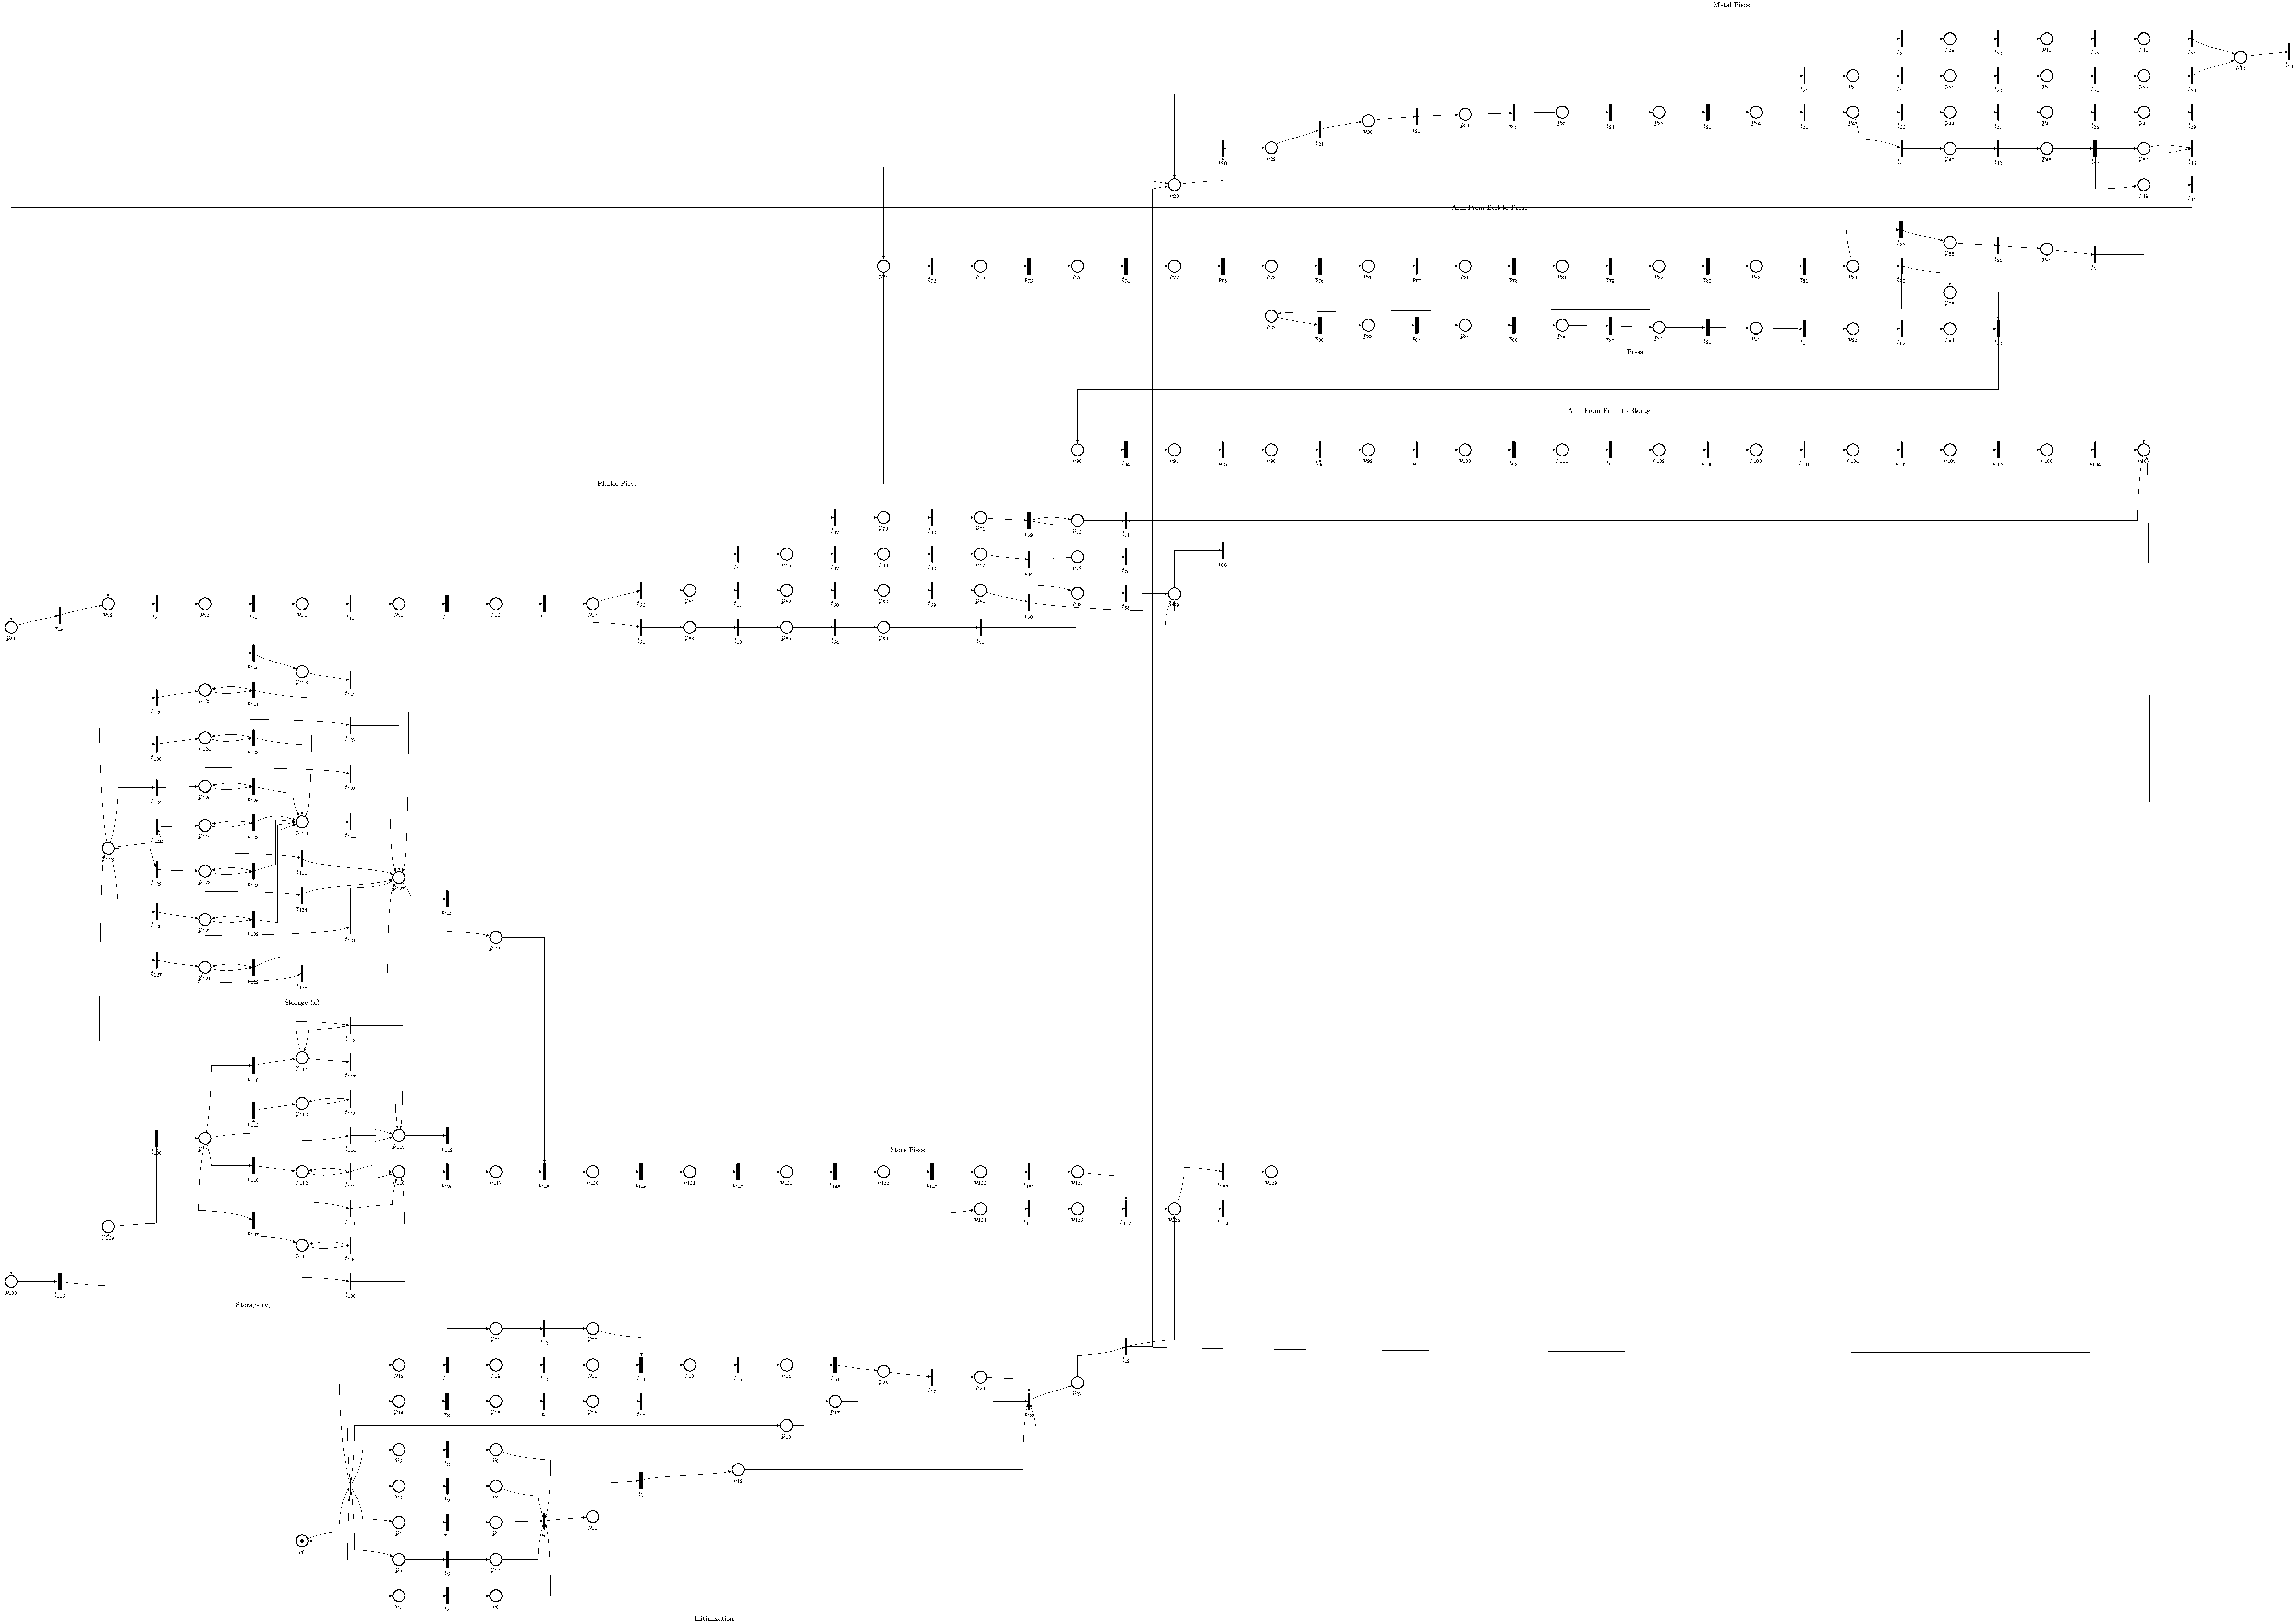
\includegraphics[height=1.28\textheight]{../../figures/petriNet/dot/complete/complete.tikz}}
% \centerline{\resizebox{!}{1.2\textheight}{\begin{tikzpicture}[>=latex',line join=bevel,]
%%
\begin{scope}
  \pgfsetstrokecolor{black}
  \definecolor{strokecol}{rgb}{1.0,1.0,1.0};
  \pgfsetstrokecolor{strokecol}
  \definecolor{fillcol}{rgb}{1.0,1.0,1.0};
  \pgfsetfillcolor{fillcol}
\end{scope}
  \node (x13) at (820.63bp,204.75bp) [draw,circle, double,place, label=above:,rotate=0] {$x_{13}$};
  \node (x12) at (623.63bp,229.75bp) [draw,,circle, label=above:,rotate=0] {$x_{12}$};
  \node (x8) at (623.63bp,531.75bp) [draw,circle, double,place, label=above:,rotate=0] {$x_{8}$};
  \node (x2) at (413.63bp,294.75bp) [draw,,circle, label=above:,rotate=0] {$x_{2}$};
  \coordinate (init) at (28.63bp,208.75bp);
  \node (x9) at (190.63bp,75.748bp) [draw,,circle, label=above:,rotate=0] {$x_{9}$};
  \node (x11) at (518.63bp,229.75bp) [draw,,circle, label=above:,rotate=0] {$x_{11}$};
  \node (x10) at (302.63bp,75.748bp) [draw,circle, double,place, label=above:,rotate=0] {$x_{10}$};
  \node (x3) at (518.63bp,363.75bp) [draw,,circle, label=above:,rotate=0] {$x_{3}$};
  \node (x0) at (93.63bp,208.75bp) [draw,,circle, label=above:,rotate=0] {$x_{0}$};
  \node (x1) at (242.63bp,358.75bp) [draw,,circle, label=above:,rotate=0] {$x_{1}$};
  \node (x6) at (190.63bp,208.75bp) [draw,,circle, label=above:,rotate=0] {$x_{6}$};
  \node (x7) at (302.63bp,234.75bp) [draw,,circle, label=above:,rotate=0] {$x_{7}$};
  \node (x4) at (715.63bp,290.75bp) [draw,,circle, label=above:,rotate=0] {$x_{4}$};
  \node (x5) at (820.63bp,376.75bp) [draw,circle, double,place, label=above:,rotate=0] {$x_{5}$};
  \draw [-Latex] (x4) ..controls (740.45bp,270.42bp) and (776.04bp,241.27bp)  .. (x13);
  \definecolor{strokecol}{rgb}{0.0,0.0,0.0};
  \pgfsetstrokecolor{strokecol}
  \draw (763.63bp,274.25bp) node {\scriptsize $\uparrow$1$\uparrow$2$\downarrow$3 \{3\}};
  \draw [-Latex] (x2) ..controls (440.38bp,278.19bp) and (476.09bp,256.08bp)  .. (x11);
  \draw (464.63bp,284.25bp) node {\scriptsize $\uparrow$1 \{3\}};
  \draw [-Latex] (x0) ..controls (125.39bp,240.72bp) and (195.71bp,311.52bp)  .. (x1);
  \draw (142.63bp,286.25bp) node {\scriptsize $\uparrow$2 \{0\}};
  \draw [-Latex] (x11) ..controls (549.13bp,229.75bp) and (579.37bp,229.75bp)  .. (x12);
  \draw (569.63bp,239.25bp) node {\scriptsize $\downarrow$1$\downarrow$2$\downarrow$3 \{3\}};
  \draw [-Latex] (x6) ..controls (219.89bp,215.54bp) and (258.12bp,224.42bp)  .. (x7);
  \draw (242.63bp,234.25bp) node {\scriptsize $\uparrow$1$\uparrow$2 \{1, 3\}};
  \draw [-Latex] (x1) ..controls (280.92bp,344.42bp) and (357.34bp,315.82bp)  .. (x2);
  \draw (302.63bp,351.25bp) node {\scriptsize $\downarrow$1$\uparrow$3 \{0\}};
  \draw [-Latex] (x0) ..controls (120.39bp,208.75bp) and (149.16bp,208.75bp)  .. (x6);
  \draw (142.63bp,218.25bp) node {\scriptsize $\downarrow$1 \{1, 3\}};
  \draw [-Latex] (init) ..controls (58.462bp,208.75bp) and (65.783bp,208.75bp)  .. (x0);
  \draw [-Latex] (x2) ..controls (440.34bp,312.3bp) and (478.01bp,337.06bp)  .. (x3);
  \draw (464.63bp,350.25bp) node {\scriptsize $\downarrow$2$\downarrow$3 \{0, 1\}};
  \draw [-Latex] (x3) ..controls (540.89bp,399.37bp) and (586.69bp,472.65bp)  .. (x8);
  \draw (569.63bp,481.25bp) node {\scriptsize $\uparrow$1 \{1\}};
  \draw [-Latex] (x12) ..controls (650.18bp,247.35bp) and (679.13bp,266.55bp)  .. (x4);
  \draw (672.63bp,280.25bp) node {\scriptsize $\uparrow$3 \{3\}};
  \draw [-Latex] (x4) ..controls (740.8bp,311.36bp) and (777.58bp,341.49bp)  .. (x5);
  \draw (763.63bp,353.25bp) node {\scriptsize $\uparrow$1$\downarrow$3 \{0\}};
  \draw [-Latex] (x9) ..controls (218.67bp,75.748bp) and (251.27bp,75.748bp)  .. (x10);
  \draw (242.63bp,85.248bp) node {\scriptsize $\uparrow$1$\downarrow$2$\downarrow$3 \{2\}};
  \draw [-Latex] (x7) ..controls (330.95bp,250.05bp) and (371.05bp,271.73bp)  .. (x2);
  \draw (361.63bp,286.25bp) node {\scriptsize $\downarrow$1$\uparrow$3 \{1, 3\}};
  \draw [-Latex] (x3) ..controls (560.69bp,348.16bp) and (653.99bp,313.59bp)  .. (x4);
  \draw (623.63bp,338.25bp) node {\scriptsize $\uparrow$3 \{0\}};
  \draw [-Latex] (x0) ..controls (116.29bp,177.68bp) and (157.03bp,121.81bp)  .. (x9);
  \draw (142.63bp,175.25bp) node {\scriptsize $\downarrow$1$\uparrow$2$\uparrow$3 \{2\}};
%
\end{tikzpicture}
}}
\end{figure}



\KOMAoptions{paper=a4,paper=portrait}
\recalctypearea

%%% Local Variables:
%%% mode: latex
%%% TeX-master: "../monografia"
%%% End:


\end{document}
